%%%BEGIN_FOLD
\documentclass{article}
\usepackage[utf8]{inputenc}
\usepackage[parfill]{parskip}
\usepackage{geometry}
\usepackage{graphicx}
\usepackage{caption}
\usepackage{amsmath}
\usepackage{makecell}
\usepackage{float}
\usepackage{subcaption}
\usepackage{bm}
%%%\usepackage{minted}
\geometry{a4paper, portrait, margin=2cm}
%%%END_FOLD
\title{TERI project, MALM and current source density inversion}
\date{Discrete constrained linear inversion}
\begin{document}
\maketitle
\graphicspath{ {./Figures/} }
\section{Introduction}
\subsection{MALM}
MALM acquisitions are performed with one current electrode connected to the plat stem and the second to soil.
The other electrodes are used to measure the distribution of the electric potential, see figure \ref{MALMscheme}.

The passive-capillary water uptake directed from the roots to the leaves bases on the continuity of the water path inside the plant.
Then, the injected current is expected to flow from the stem to roots through this water continuum.
The active roots becomes the connection between the plant electrode and the soil electrode, they behave as current sources.

\begin{figure}[h]
	\centering
	\captionsetup[sub]{margin=0.4cm}
	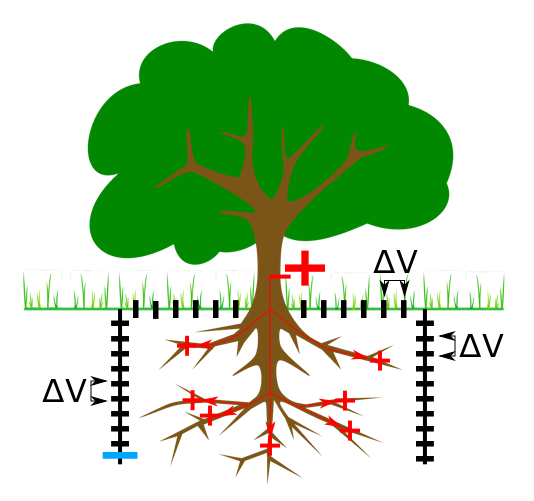
\includegraphics[width=9cm]{MALM.png}
	\caption{Possible 2D MALM configuration with boreholes. One current electrode is connected to the plant trunk (red plus), the second current electrode is chosen among the electrodes in the soil (blue minus). All the other electrodes are used to acquired potential differences and characterize the distribution of the electric potential about the rhizosphere. Soil electrodes can be placed on the surface and/or in the soil trough the use of boreholes. The current electrode in the soil can be changed in order to acquire multiple sets and improve the information on the position of the roots.\label{MALMscheme}}
\end{figure}


The distribution of the so generated electric voltage depends on:
\begin{itemize}
\item Soil conductivity distribution
\item Position of the soil electrode
\item Boundaries of the system
\item Position of the roots
\end{itemize}

The soil conductivity is derived from a normal ERT acquisition and inversion.
The position of the soil electrode is known. The system boundaries are also known, e.g., lab 3D geometry or field semi-infinite conditions.
It is then possible to infer the last factor, the unknown position of the roots.

\subsection{Current Source Density estimation}
The estimation of the current source distribution is performed on a grid of virtual electrodes (VRTe).
The VRTe are the possible sources of current that the inversion process is going to test, the result of the inversion represents the fraction of current associated with each VRTe.

All the VRTe are added as nodes to the mesh used by the ERT inversion code (BERT).
For linearity, we can sum the effects of different sources; this means we can calculate the response for each tested VRTe and define how much it is contributing to the distribution of potential measured in the LAB data. Physically this is a projection of a \textit{linear} system components.

Single or all in once??
It is technically and numerically possible to account for multiple sets of MALM data, each one acquired with a different soil electrode.
This would strongly improve the resolution of the iCSD. For example, having a set of soil electrodes around the expected position of the roots.
However, if the distribution of the current among the roots depends on the soil return electrode position it is will generate different current source distributions for each soil electrode used. Clearly, this would make more difficult the combination of different data sets.

Abbreviations:\newline
VTRe = virtual electrode, tested source; R = resistance; SOILe = real-lab electrode fixed current electrode in the soil

Our goal is to estimate the VRTe current fractions from the VRTe simulated $\Delta$P and the measured resistances.

\section{BERT calculation of the VRTe responses}

\subsection{Mesh}

Add virtual (VRTe) electrodes to the BERT mesh. Then, the mesh contains both the real electrodes, which are used for the potential differences and for the return electrode, and the VRTe, which are used for the current injection.

\begin{figure*}[p]
	\centering
	\captionsetup[sub]{margin=0.4cm}
	\subcaptionbox{Rhizotron geometry and electrodes (1:64).\label{Rhizotron}}{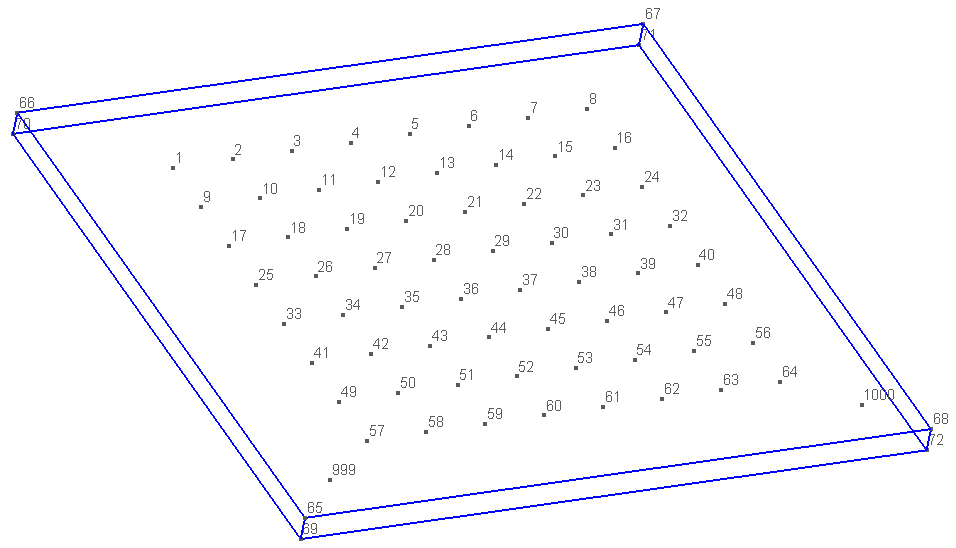
\includegraphics[width=8cm]{BERT_Fiat_electrodes.png}}
	\subcaptionbox{Local refinement.\label{Local}}{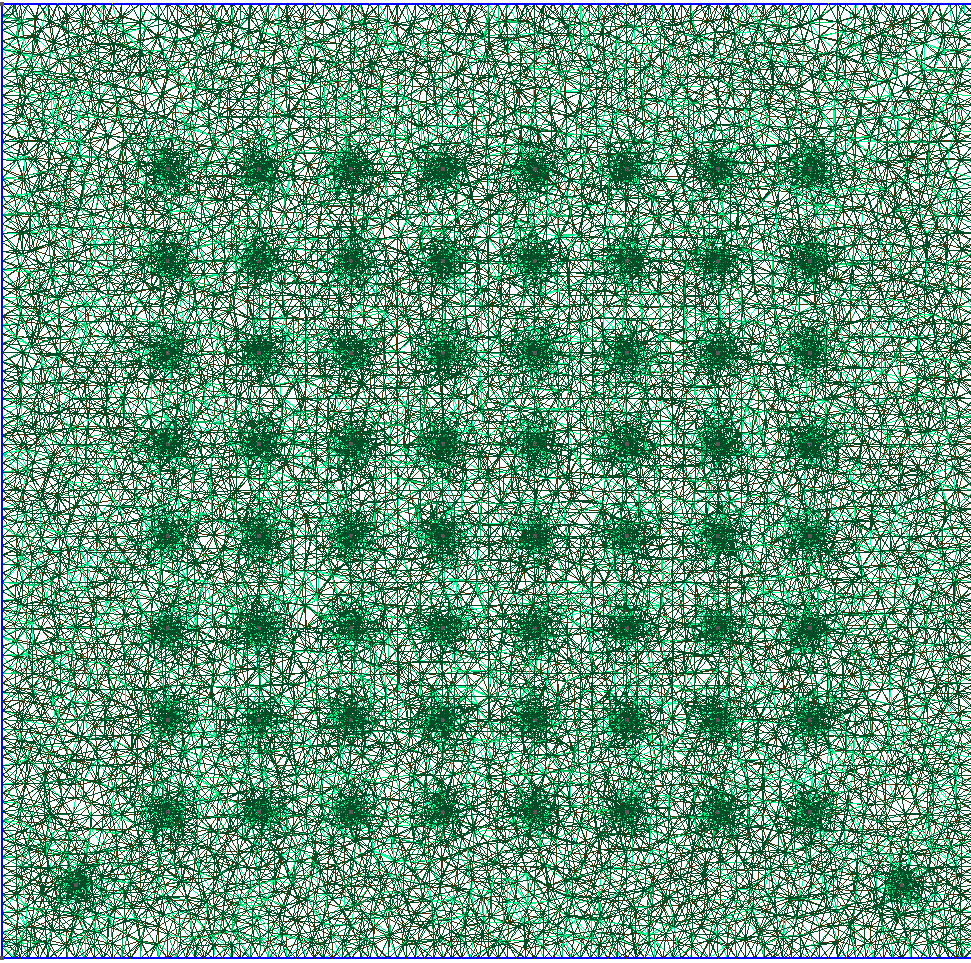
\includegraphics[width=8cm]{BERT_Fiat.png}}
	\subcaptionbox{Check mesh quality.\label{MeshQuality}}{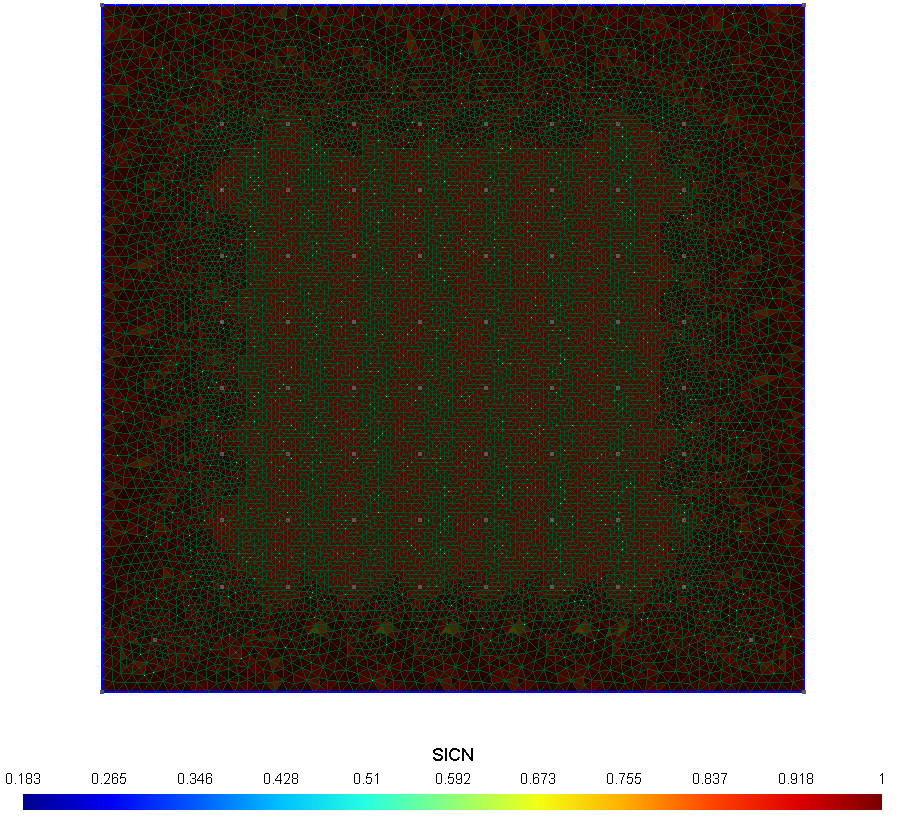
\includegraphics[width=8cm]{BERT_NoRef_quality.png}}
	\subcaptionbox{Distributed refinement.\label{Distributed}}{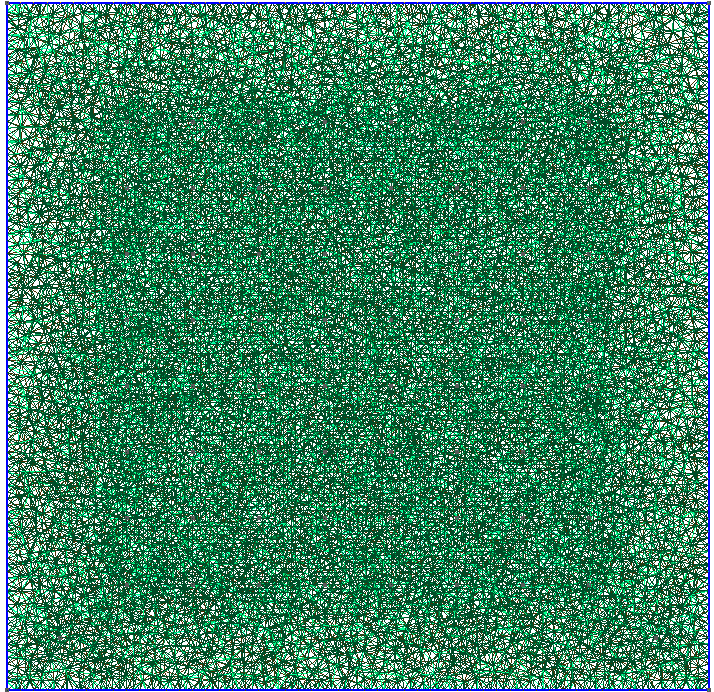
\includegraphics[width=8cm]{BERT_NoRef.png}}
	\caption{Mesh preparation.\label{RhiMesh}}
\end{figure*}

\subsection{Sequence}

VRTe1 SOILe1 M1 N1\newline
VRTe1 SOILe1 M2 N2\newline
...\newline
VRTe1 SOILe1 Mlast Nlast\newline
"""\newline
VRTe2 SOILe1 M1 N1\newline
VRTe2 SOILe1 M2 N2\newline
...\newline
VRTe2 SOILe1 Mlast Nlast\newline
"""\newline
VRTe3 SOILe1 M1 N1\newline
VRTe3 SOILe1 M2 N2\newline
...\newline
VRTe3 SOILe1 Mlast Nlast\newline
...etc...
VRTe1 SOILe2 M1 N1\newline
VRTe1 SOILe2 M2 N2\newline
...\newline
VRTe1 SOILe2 Mlast Nlast\newline
"""\newline
VRTe2 SOILe2 M1 N1\newline
VRTe2 SOILe2 M2 N2\newline
...\newline
VRTe2 SOILe2 Mlast Nlast\newline
"""\newline
VRTe3 SOILe2 M1 N1\newline
VRTe3 SOILe2 M2 N2\newline
...\newline
VRTe3 SOILe2 Mlast Nlast\newline
...etc...

Run forward model on the inverted resistivity model, one single sequence can contain all the possible sources.

As the forward simulation run only once, it is possible to use a very fine mesh. This can be done using \textit{secMesh.bms} and a rho.map extracted from the \textit{fop-model.vtk}.

\section{Least squares inversion}

The least squares method is adopted to estimates the current fraction associated with each VRTe.

Spatial regularization, current conservation and parameters boundaries are added to the least squares problem. A specific and adjustable weight is given to each of these constrains to control the trade-off between data fitting and regularization.

\subsection{Linear system}

Because of its linearity, the inverse problem can be expressed as $\bm{Ax=b}$. Where $\bm{A}$ is the model, a matrix containing the VRTe simulated responses and the regularization; $\bm{x}$ is a vector containing the model parameters to be estimated, the VRTe current fractions; and $\bm{b}$ is a vector containing the observed data and regularization targets.

The simulated VRTe responses are organized into the $\bm{A}$ matrix, each VRTe response being a column. Therefore, the number of columns of $\bm{A}$ corresponds to the number of VRTes.

Each row in $\bm{A}$ expresses the contributions of the VRTes to the relative data in $\bm{b}$. Therefore, the number of rows in $\bm{A}$ corresponds to the number of observed data in $\bm{b}$.

\subsection{Current conservation constrain}

Because of the current conservation, the condition that the sum of all the current fractions is equal to 1 has to be respected. In this way, the total injected current will be consistently returned by the return electrode, whose intensity is normalized to -1.

This condition can be included into least squares problem by adding a new all-ones row to the $\bm{A}$ matrix. The new row represents the sum of all the elements in the column $\bm{x}$, which is set to be equal to 1 by adding this value as new element to the column $\bm{b}$.

\subsection{Spatial regularization}

A 2D spatial regularization is implemented to stabilize the numerical inversion and control the trade-off between solution roughness and data fit. As for the previous constrain, this condition is included into the least squares problem by adding new rows to the $\bm{A}$ matrix.

Each new row expresses a first order finite difference between two consecutive VRTes, -1 and 1 are inserted in the columns of the 2 VRTes considered. The difference is set to be equal to 0 by adding this new entry into the column $\bm{b}$.

\resizebox{\textwidth}{!}{$\displaystyle
\begin{array}{cccccc}
\bm{W}&\bm{A}&\bm{x}& & \bm{b} & \bm{W}\\[0.2cm]
\begin{pmatrix}
W_{obs} & 0 & \cdots & 0 \\
0 & w_{obs} & \cdots & 0 \\
\vdots & \vdots & \ddots & \vdots \\
0 & 0 & \cdots & w_{reg}
\end{pmatrix}
&\begin{pmatrix}
S_1R_1 & S_2R_1 & \cdots & S_nR_1 \\
S_1R_2 & S_2R_2 & \cdots & S_nR_2 \\
\vdots  & \vdots  & \ddots & \vdots  \\
S_1R_m & S_2R_m & \cdots & S_nR_m\\
1 & 1 & \cdots & 1 \\
-1 & 1 & \cdots & 0\\
0 & -1 & \cdots & 0 \\
\vdots & \vdots & \ddots & \vdots \\
0 & 0 & \cdots & 1 \\
\end{pmatrix}
&\begin{pmatrix}
S_{1,cf} \\
S_{2,cf} \\
\vdots \\
S_{n,cf} \end{pmatrix}
& =
& \begin{pmatrix}
R_{1,meas} \\
R_{2,meas} \\
\vdots \\
R_{m,meas}\\
1\\
0\\
0\\
\vdots\\
0\\
\end{pmatrix}
&\begin{pmatrix}
W_{obs} & 0 & \cdots & 0 \\
0 & w_{obs} & \cdots & 0 \\
\vdots & \vdots & \ddots & \vdots \\
0 & 0 & \cdots & w_{reg}
\end{pmatrix}
\end{array}$}


\subsection{Constrain and regularization weights}

The weight of the different observations and constrains can be modified by multiplying both $\bm{A}$ and $\bm{b}$ a weighting diagonal matrix. In this way, a small misfit relative to the target value is forced, where desired, by increasing its absolute value compared to the other observations and/or constrains.

After the inversion, the residuals of the unweighted problem can still be obtained. The residuals of the weighted least squares solution are divided by the weights, the so obtained unweighted residuals can then be better analyzed and compared. For example to construct the L-curve.

\subsection{L-curve and optimal regularization}

In order to identify the optimum value for the regularization weights, the model-to-data fit can be compared with the solution roughness. This is done by performing several least squares inversion with different regularization weights and plotting the solution roughness against the data fit. The solution roughness is defined as the sum of the unweighted regularization residuals, that is how the model deviates from the regularized target. The obtain curve, called L-curved, illustrates how the model-to-data fit decreases while increasing the regularization.

\begin{figure}[H]
	\centering
	\captionsetup[sub]{margin=0.4cm}
	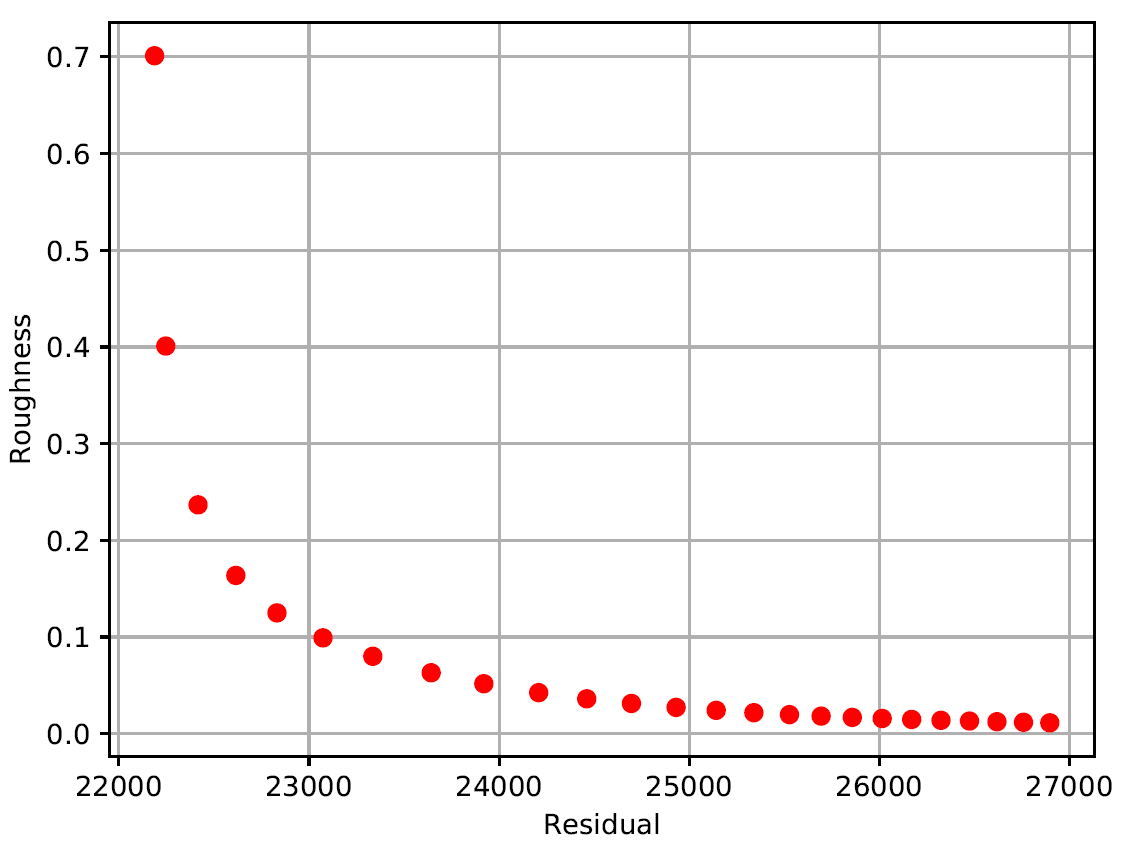
\includegraphics[width=8cm]{L_curve.png}
	\caption{Trade-off between model-to-data fit and regularization.\label{Lcurve}}
\end{figure}

The L-curve allows to understand at which point the model-to-fit improvement is minimal and does not justify the associated increment of the solution roughness. The optimum level of regularization is that at which the curve deflects sharply upwards, that is the solution deviates from the regularization conditions without a significant improvement of the data fit.

\subsection{Bounding values}

The weighted linear problem is solved with the use of a python library that offers two different numerical algorithms. Both algorithms solves the linear system in the least-squares sense and allows the definition of variable boundaries. An implementation of a subspace trusted region method proposed by Branch et al., 1999, has been used for the current inversion.

\subsection{Comparison with PEST}

PEST is a standard software package for parameter estimation and numerical uncertainty. PEST was initially used for the current source density inversion, but the present and specific code offers two main advantages:

\begin{itemize}
	\item Take advantage of the problem linearity. PEST is designed to solved nonlinear problems, such as hydraulic or resistivity distribution. As consequence, PEST does not account for the problem linearity and calculates the Jacobian matrix at each iteration. The calculation of the Jacobian matrix requires, without linearity assumption, PEST to externally call the physical forward model at least as many times as there are adjustable parameters (VRTe). The specific number of calls depends on the type of derivative used, and may need to be increased to obtain higher resolution and reduce rounding errors. For each model call PEST writes the modified parameters and reads the model results through text files. As consequence of the many model calls and write/read time, the inversion time significantly increases.
	\item  In order to facilitate the  problem definition PEST takes care of the matrices preparation. The user defines the problem to solve through a list of commands and inputs in a series of configuration files. While this allows the user to work on a higher level, it necessarily introduce an overhead of commands make it difficult to automatize the inversion procedure compared to the direct definition of the problem in matrix form.
\end{itemize}

Because of its reliability, user-friendliness, and extensive documentation, PEST represented an optimal starting point and provided the necessary initial numerical validation.

\section{Numerical and laboratory tests}
The ERT inversion quality was evaluated first. Different type of meshes were tested because of the particular rhizotron geometry (we used \textit{gmsh}).

Three initial MALM synthetic tests were performed on a homogeneous distribution of conductivity, i.e. running the forward model on the rhizotron geometry with a homogeneous resistivity of 1 Ohm/m.
In the first test the current source was placed close to a VRTe to evaluate if the inversion could properly concentrate on that VRTe the source of current. In the second test the current source was placed in a position that forced the inversion to more equally distribute the current. In the third test a vertical diffuse source of current was simulated by combining 5 sources.

Following the synthetic tests, a first laboratory experiment was performed by filling the rhizotron with only water and dropping a wire representing the roots from the top of the rhizotron. A single electrode was connected at the end of the wire. The ERT inversion produced an homogeneous distribution of resistivity (3.7 Ohm/m). Before the MALM acquisition and inversion, we tested the capability of the inverted model to reproduce the LAB data, this is important in order to evaluate if the sensitivity of the data could support the investigation of a current source.

\begin{figure}
	\centering
	\captionsetup[sub]{margin=0.4cm}
	\subcaptionbox{Source concentrated on one VRTe.\label{S2NMiCSD}}{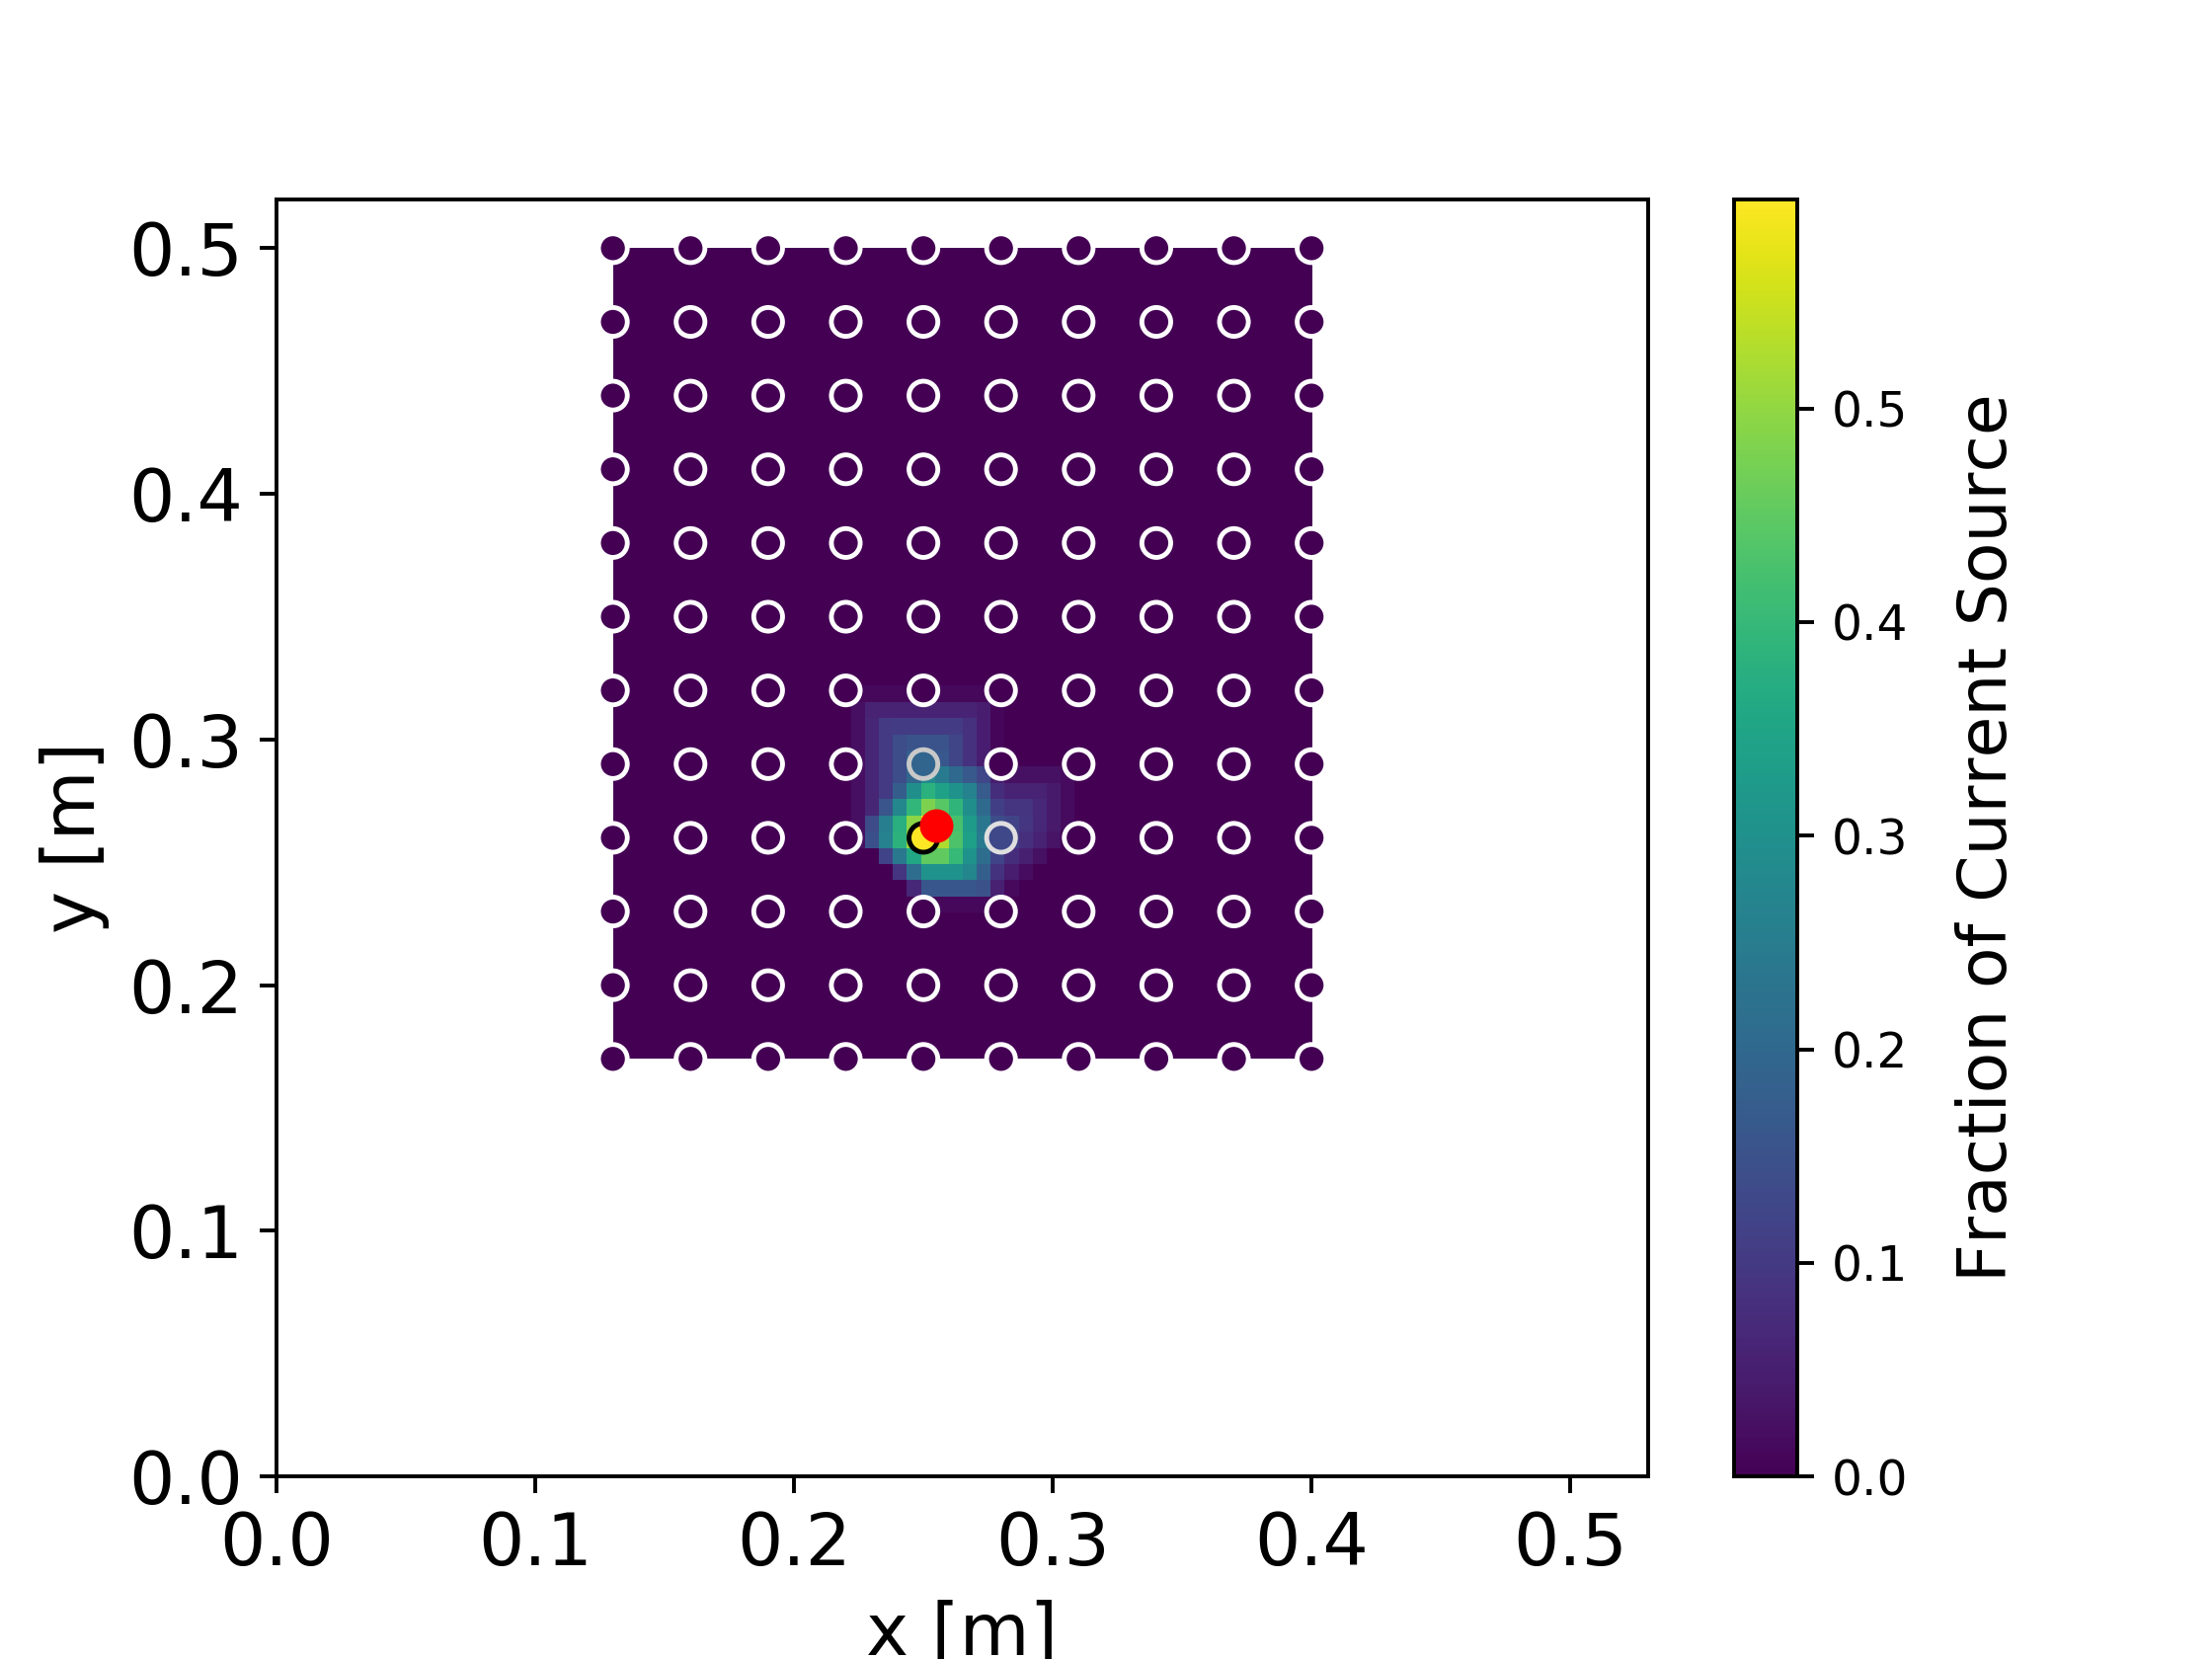
\includegraphics[width=5.5cm]{S2NMiCSD.png}}
	\subcaptionbox{Source distributed among the 4 closest VRTe. \label{S1NMiCSD}}{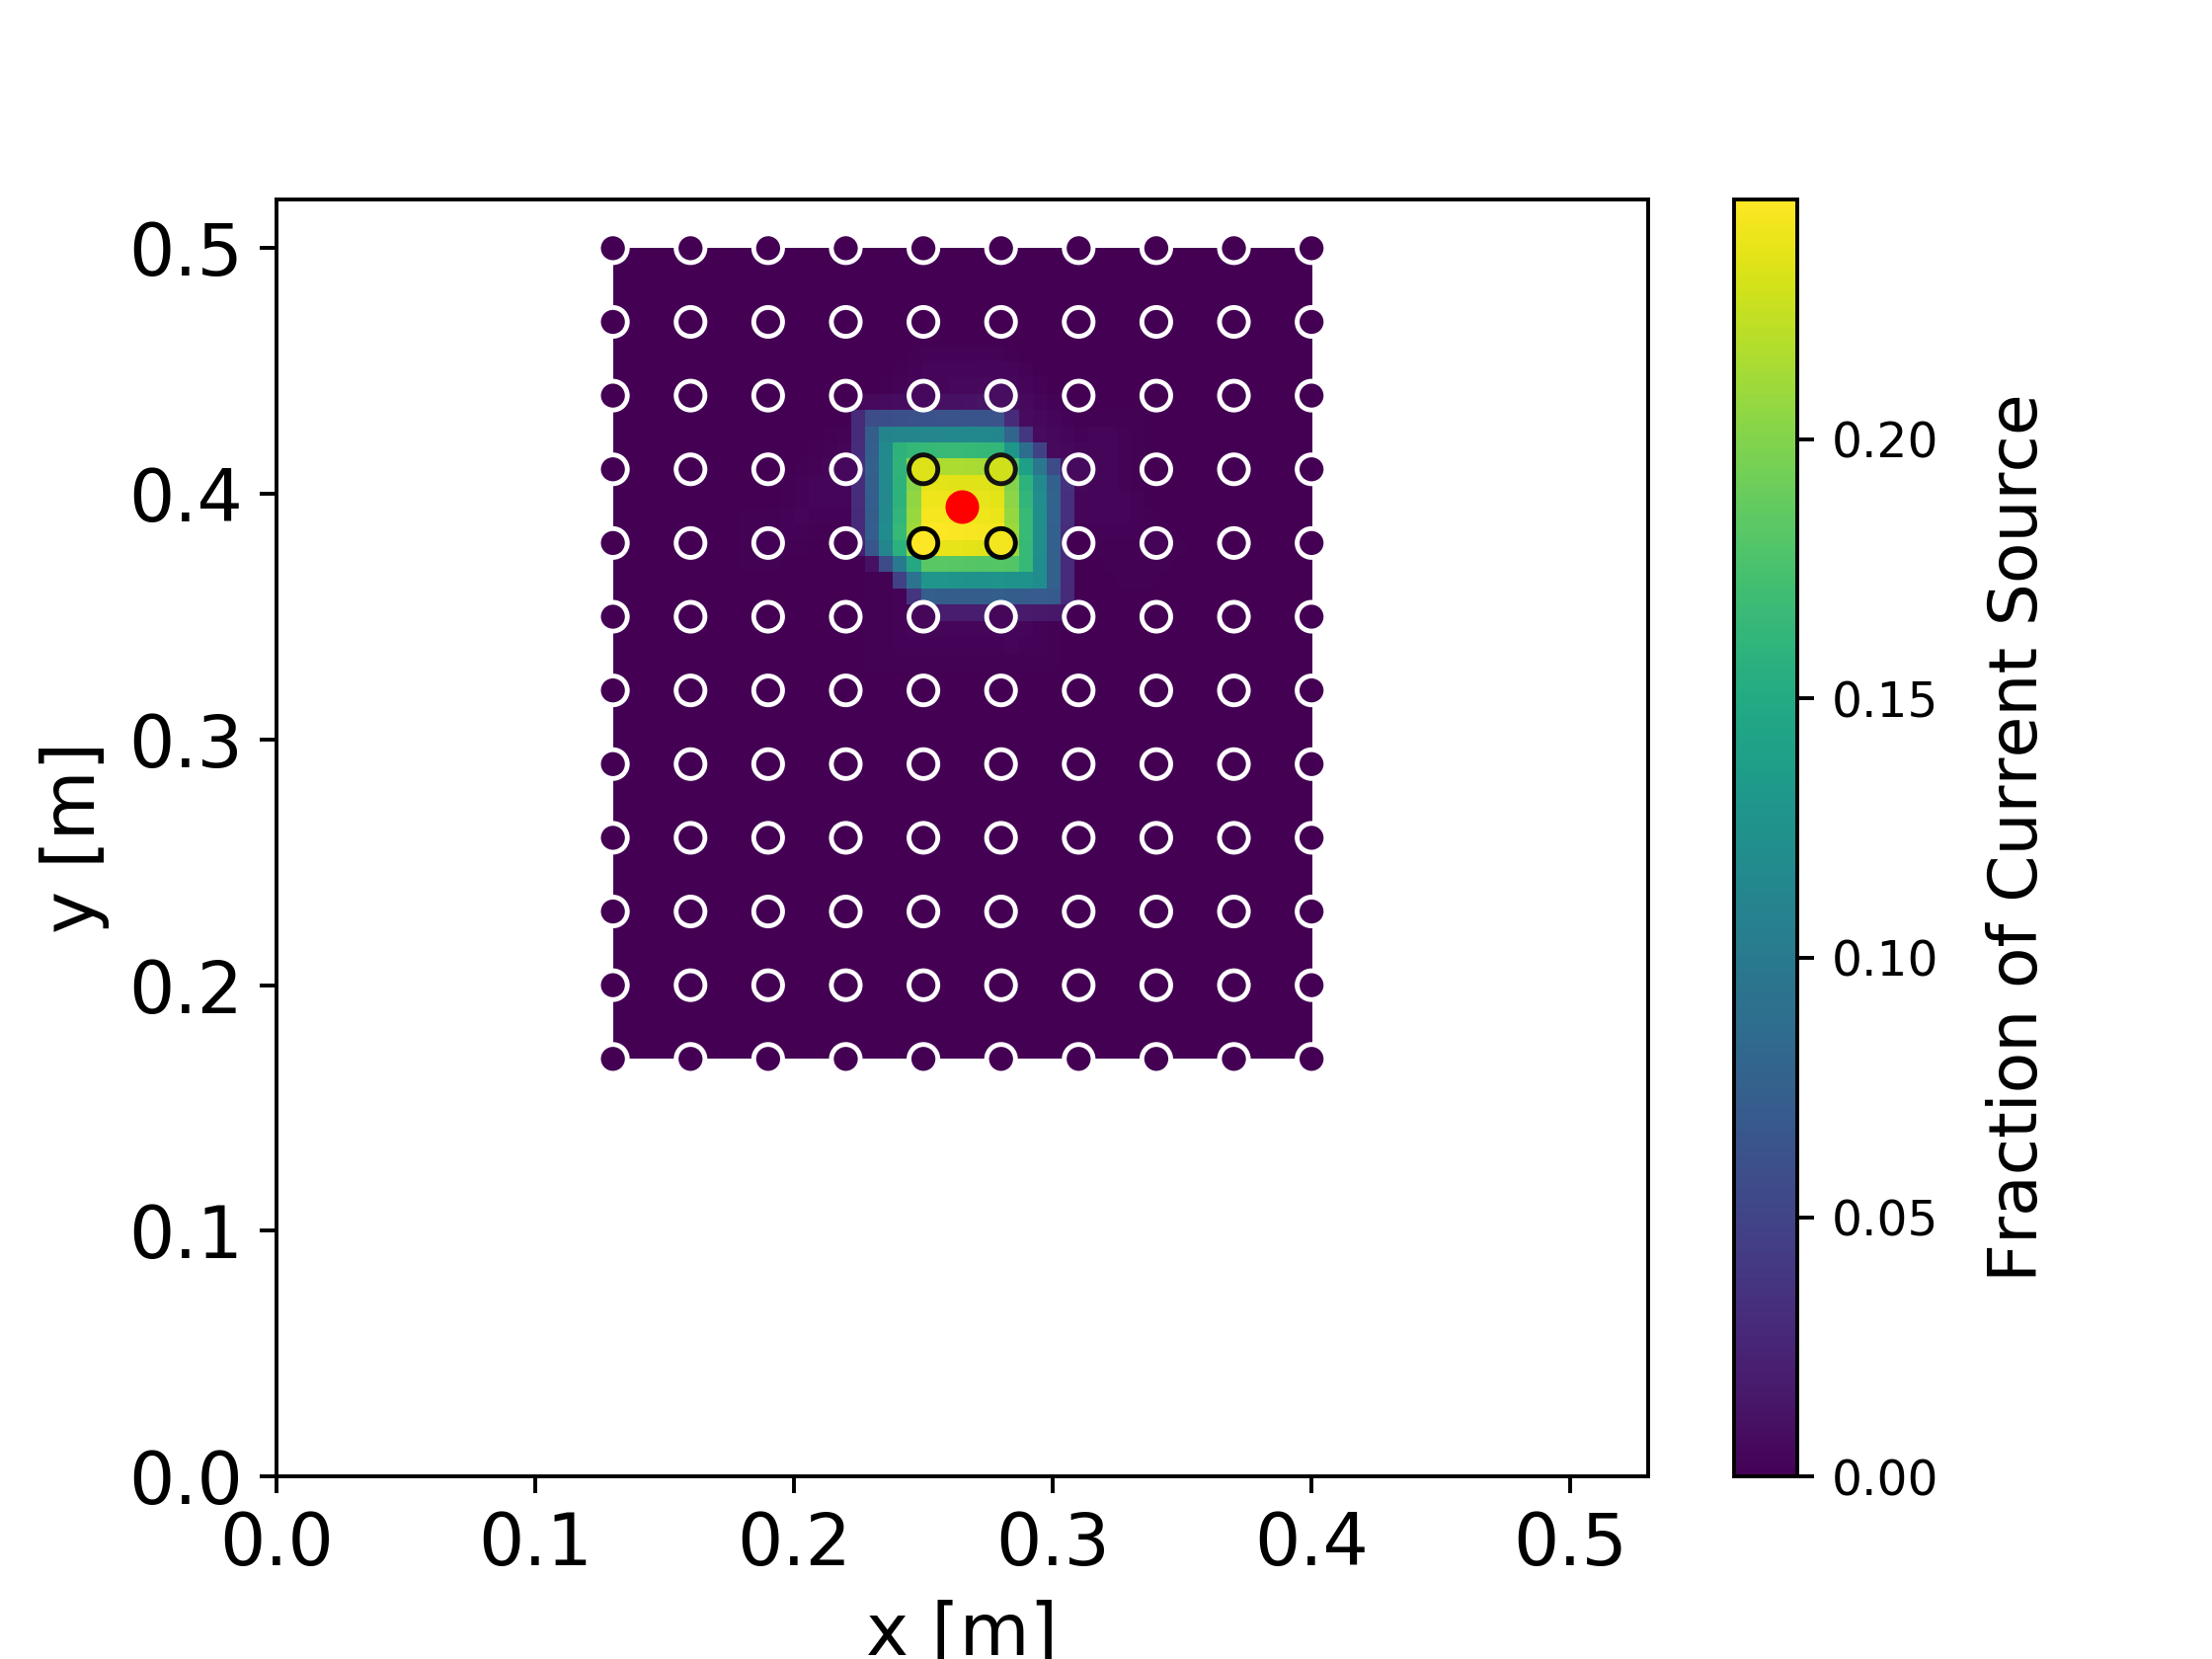
\includegraphics[width=5.5cm]{S1NMiCSD.png}}
	\subcaptionbox{Distributed source. \label{SMultiple}}{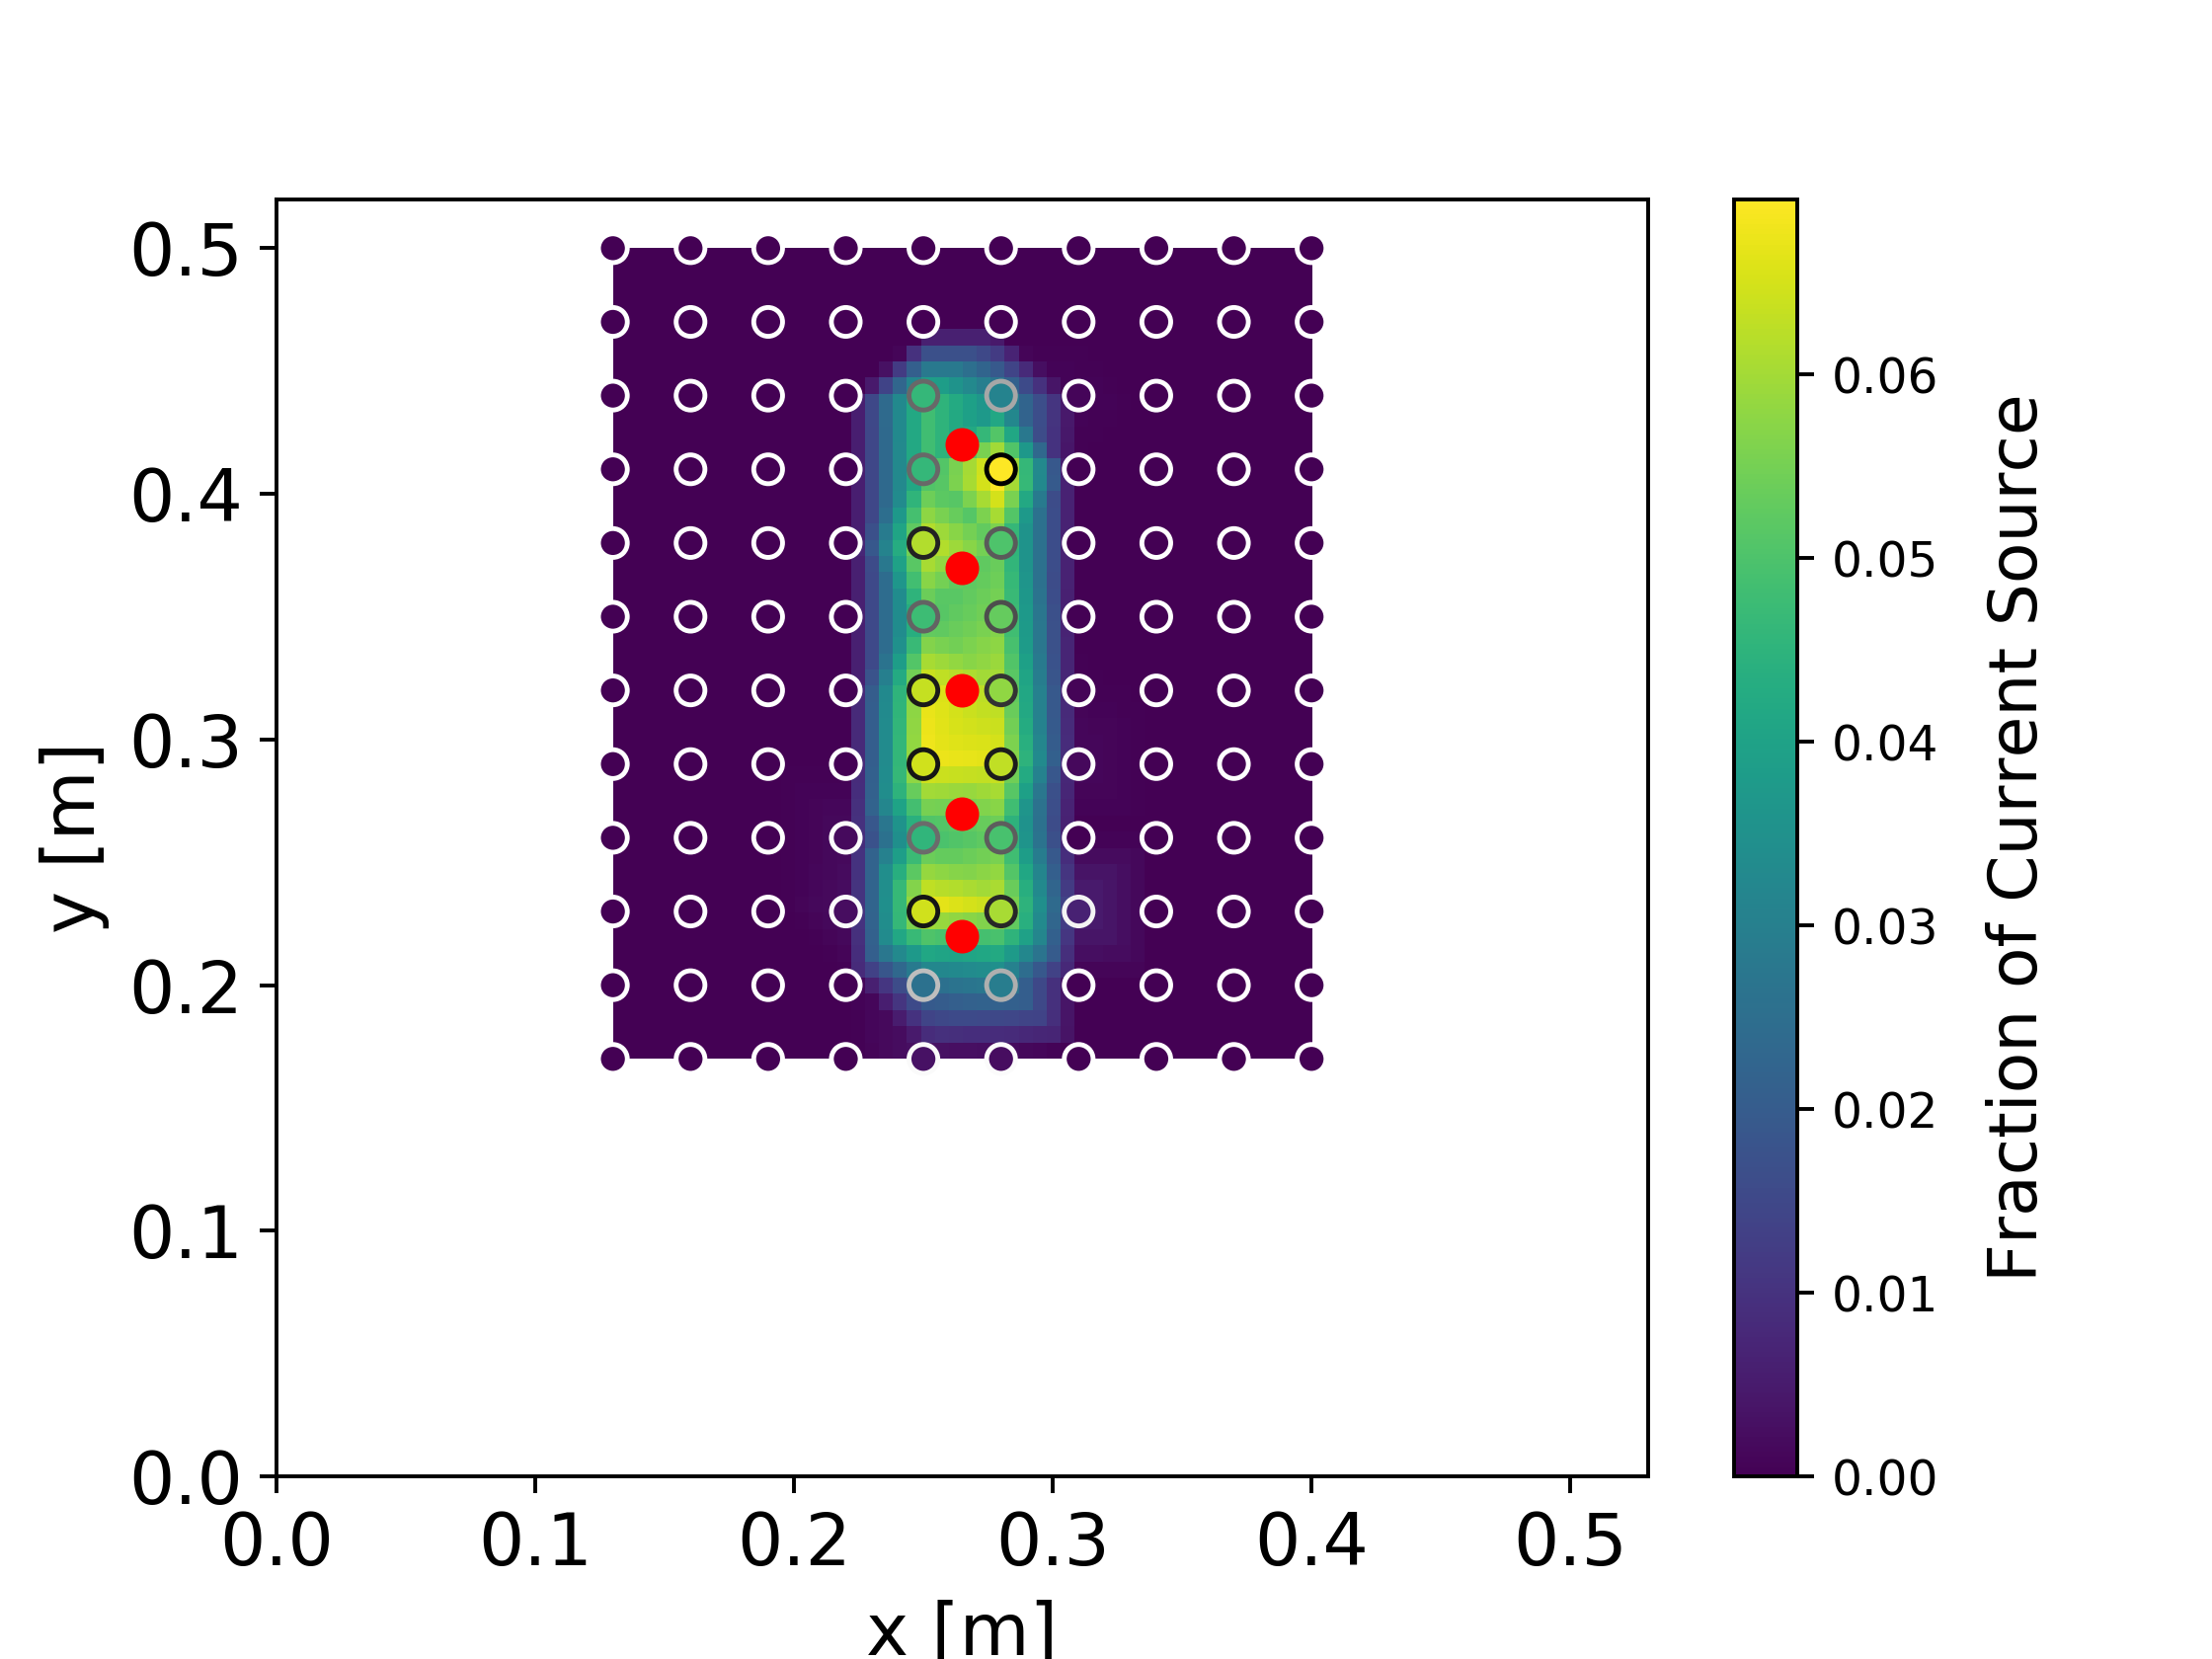
\includegraphics[width=5.5cm]{SMultiple.png}}
	\caption{Synthetic models, linear interpolation of the current fraction associated with the VRTe.\label{SynSCD}}
\end{figure}

\begin{figure}[b]
	\centering
	\captionsetup[sub]{margin=0.4cm}
	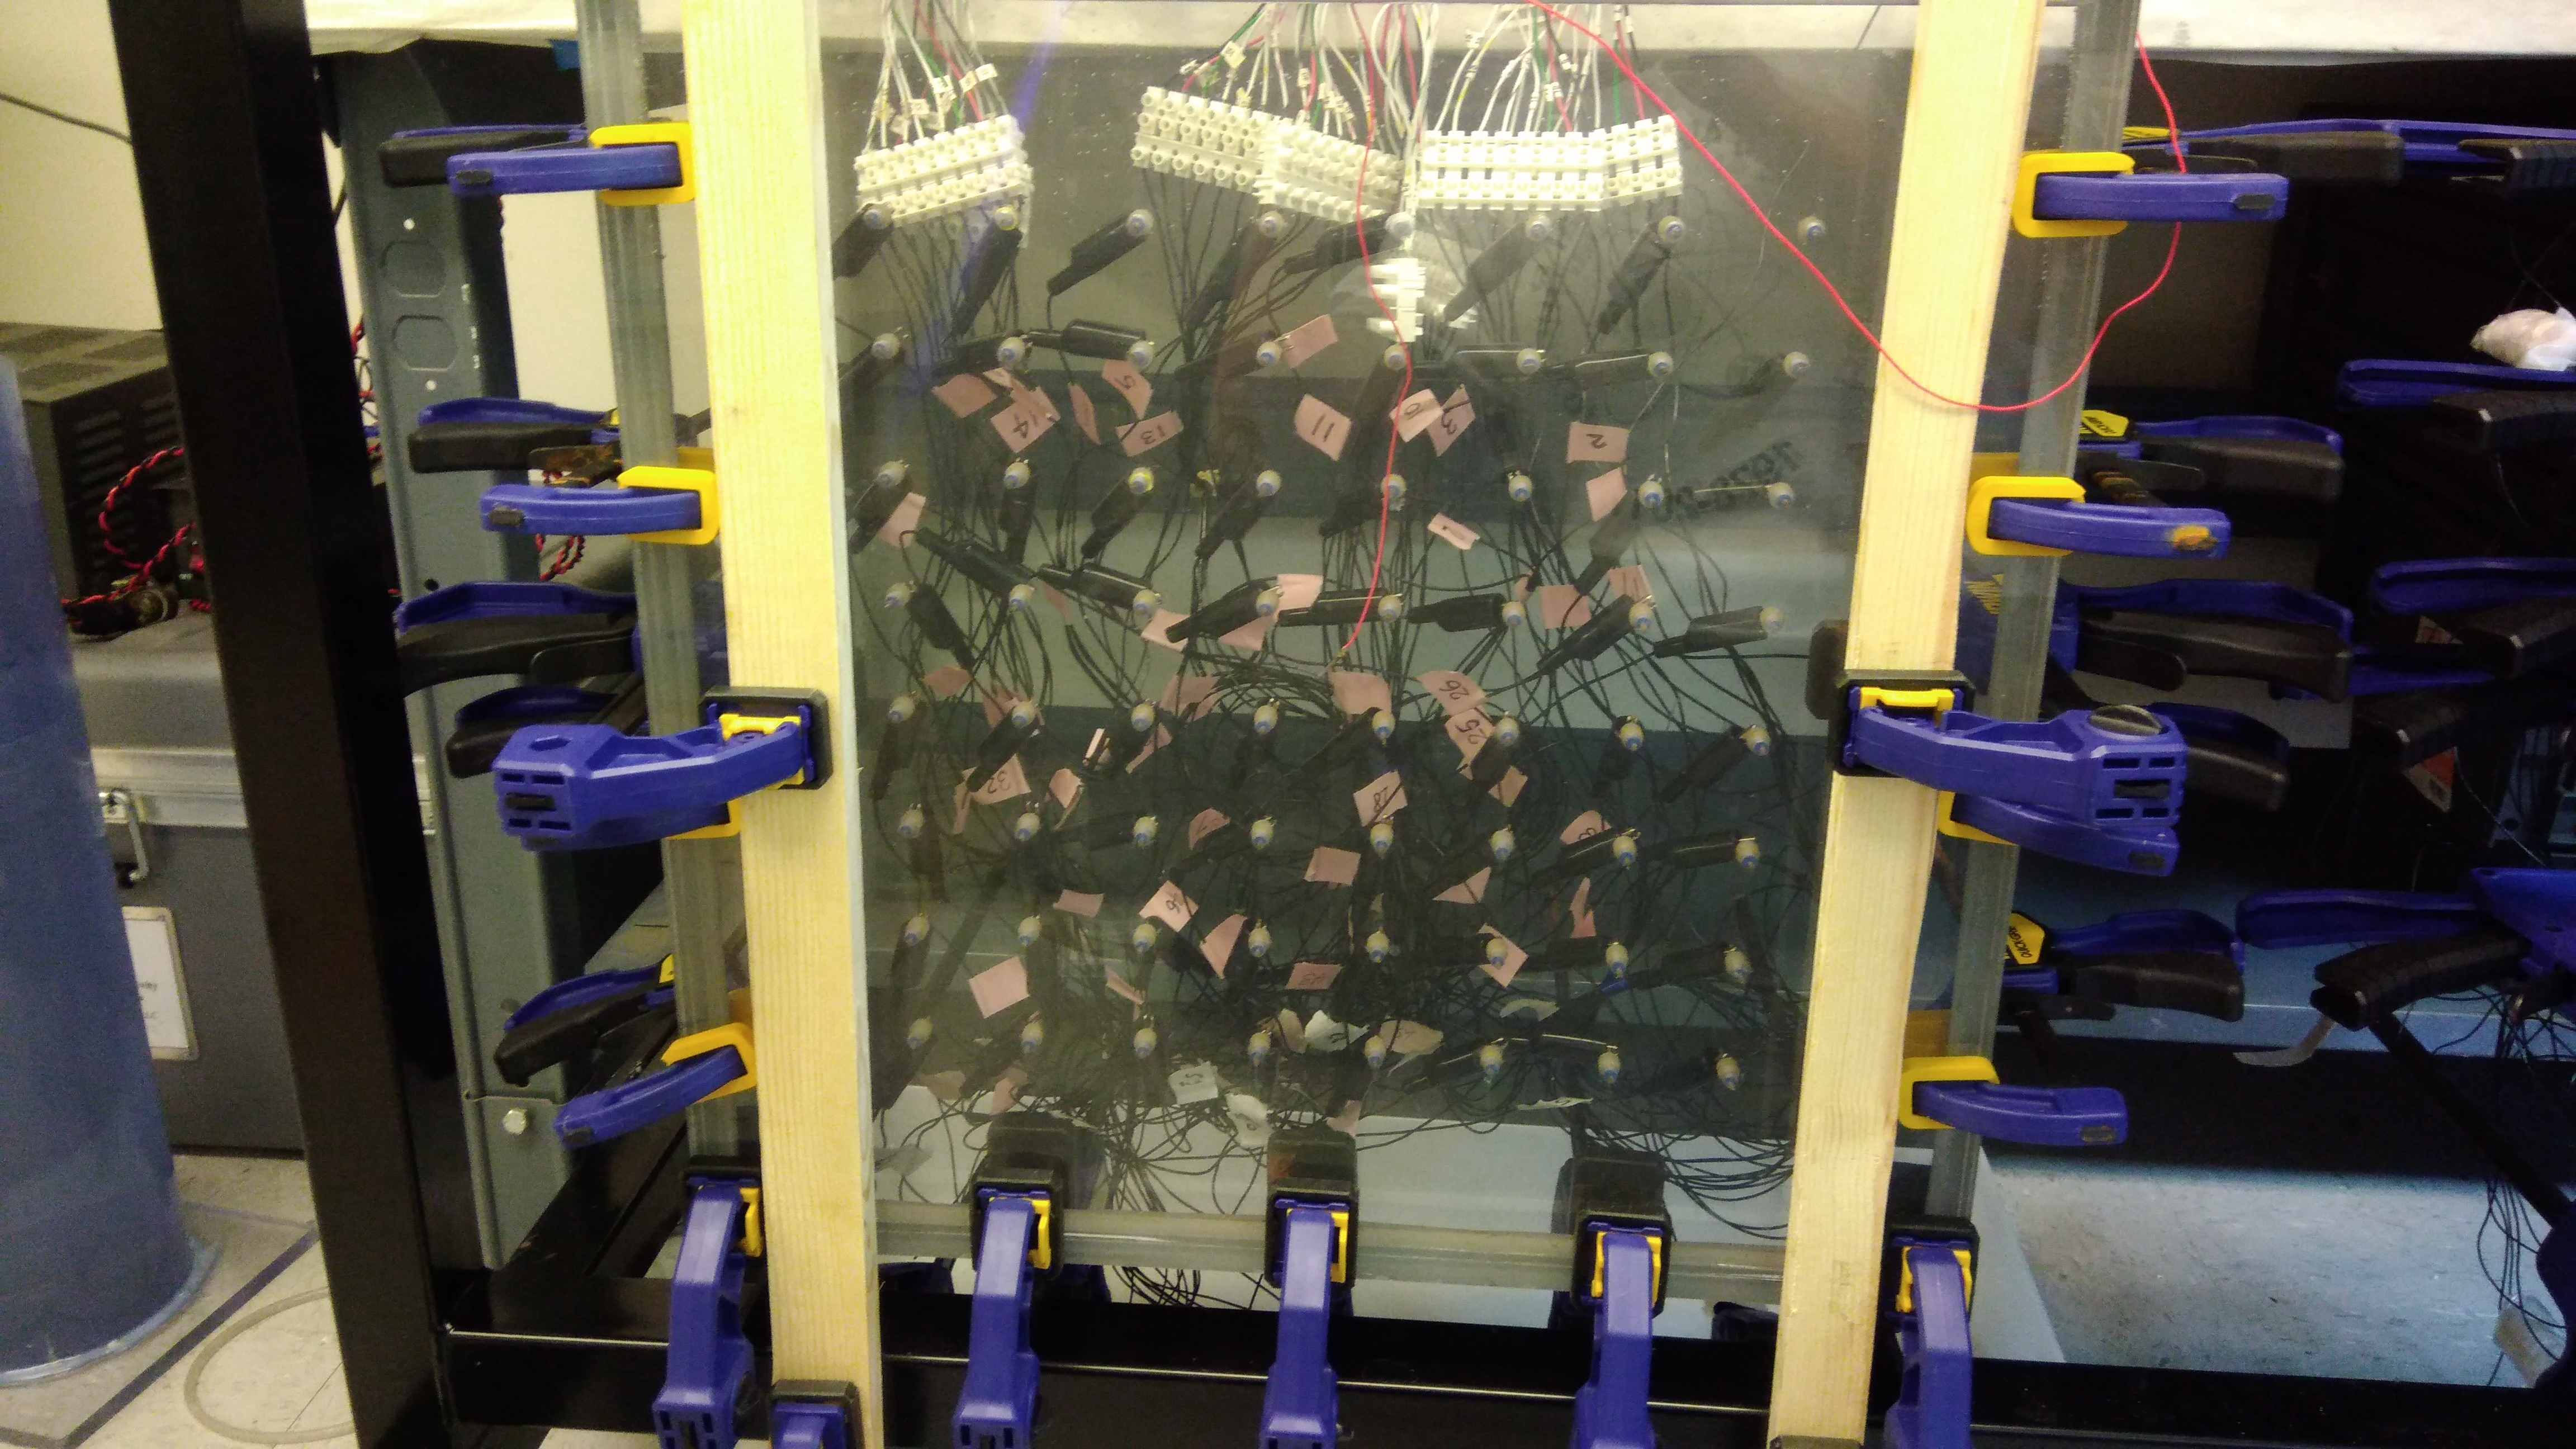
\includegraphics[width=9cm]{MALM_Labtest.jpg}
	\caption{MALM configuration for the lab test, the red cable supplies a small injection electrode positioned in the center of the rhizotron.\label{LabMALM}}
\end{figure}
\begin{figure}
	\centering
	\captionsetup[sub]{margin=0.4cm}
	\subcaptionbox{Inverted resistivity distribution.\label{ERTmodel}}{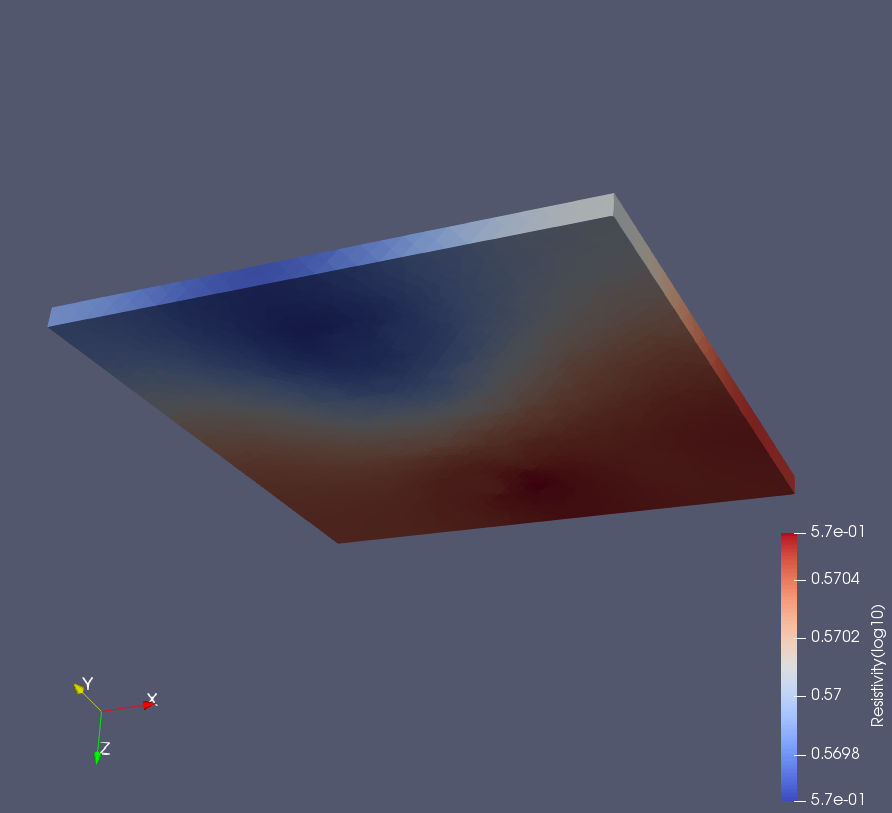
\includegraphics[width=8cm]{ERT4MALM2.png}}
	\subcaptionbox{ERT data check, comparison between laboratory ERT data and resistances modeled on the inverted resistivity model.\label{LabSynComp}}{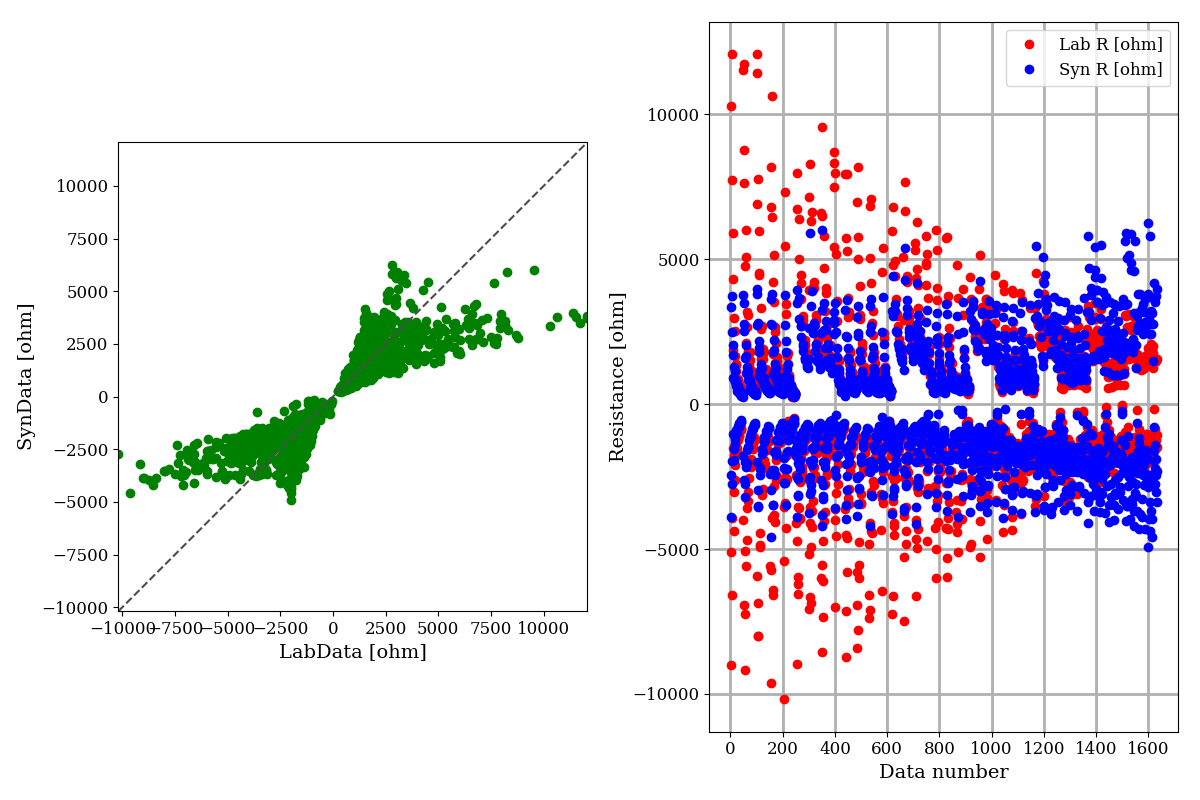
\includegraphics[width=8.5cm]{LabSynComparison.png}}
	\subcaptionbox{Estimated current source distribution, the red point represents the position of the electrode inside the rhizotron in the laboratory.\label{LabSCD}}{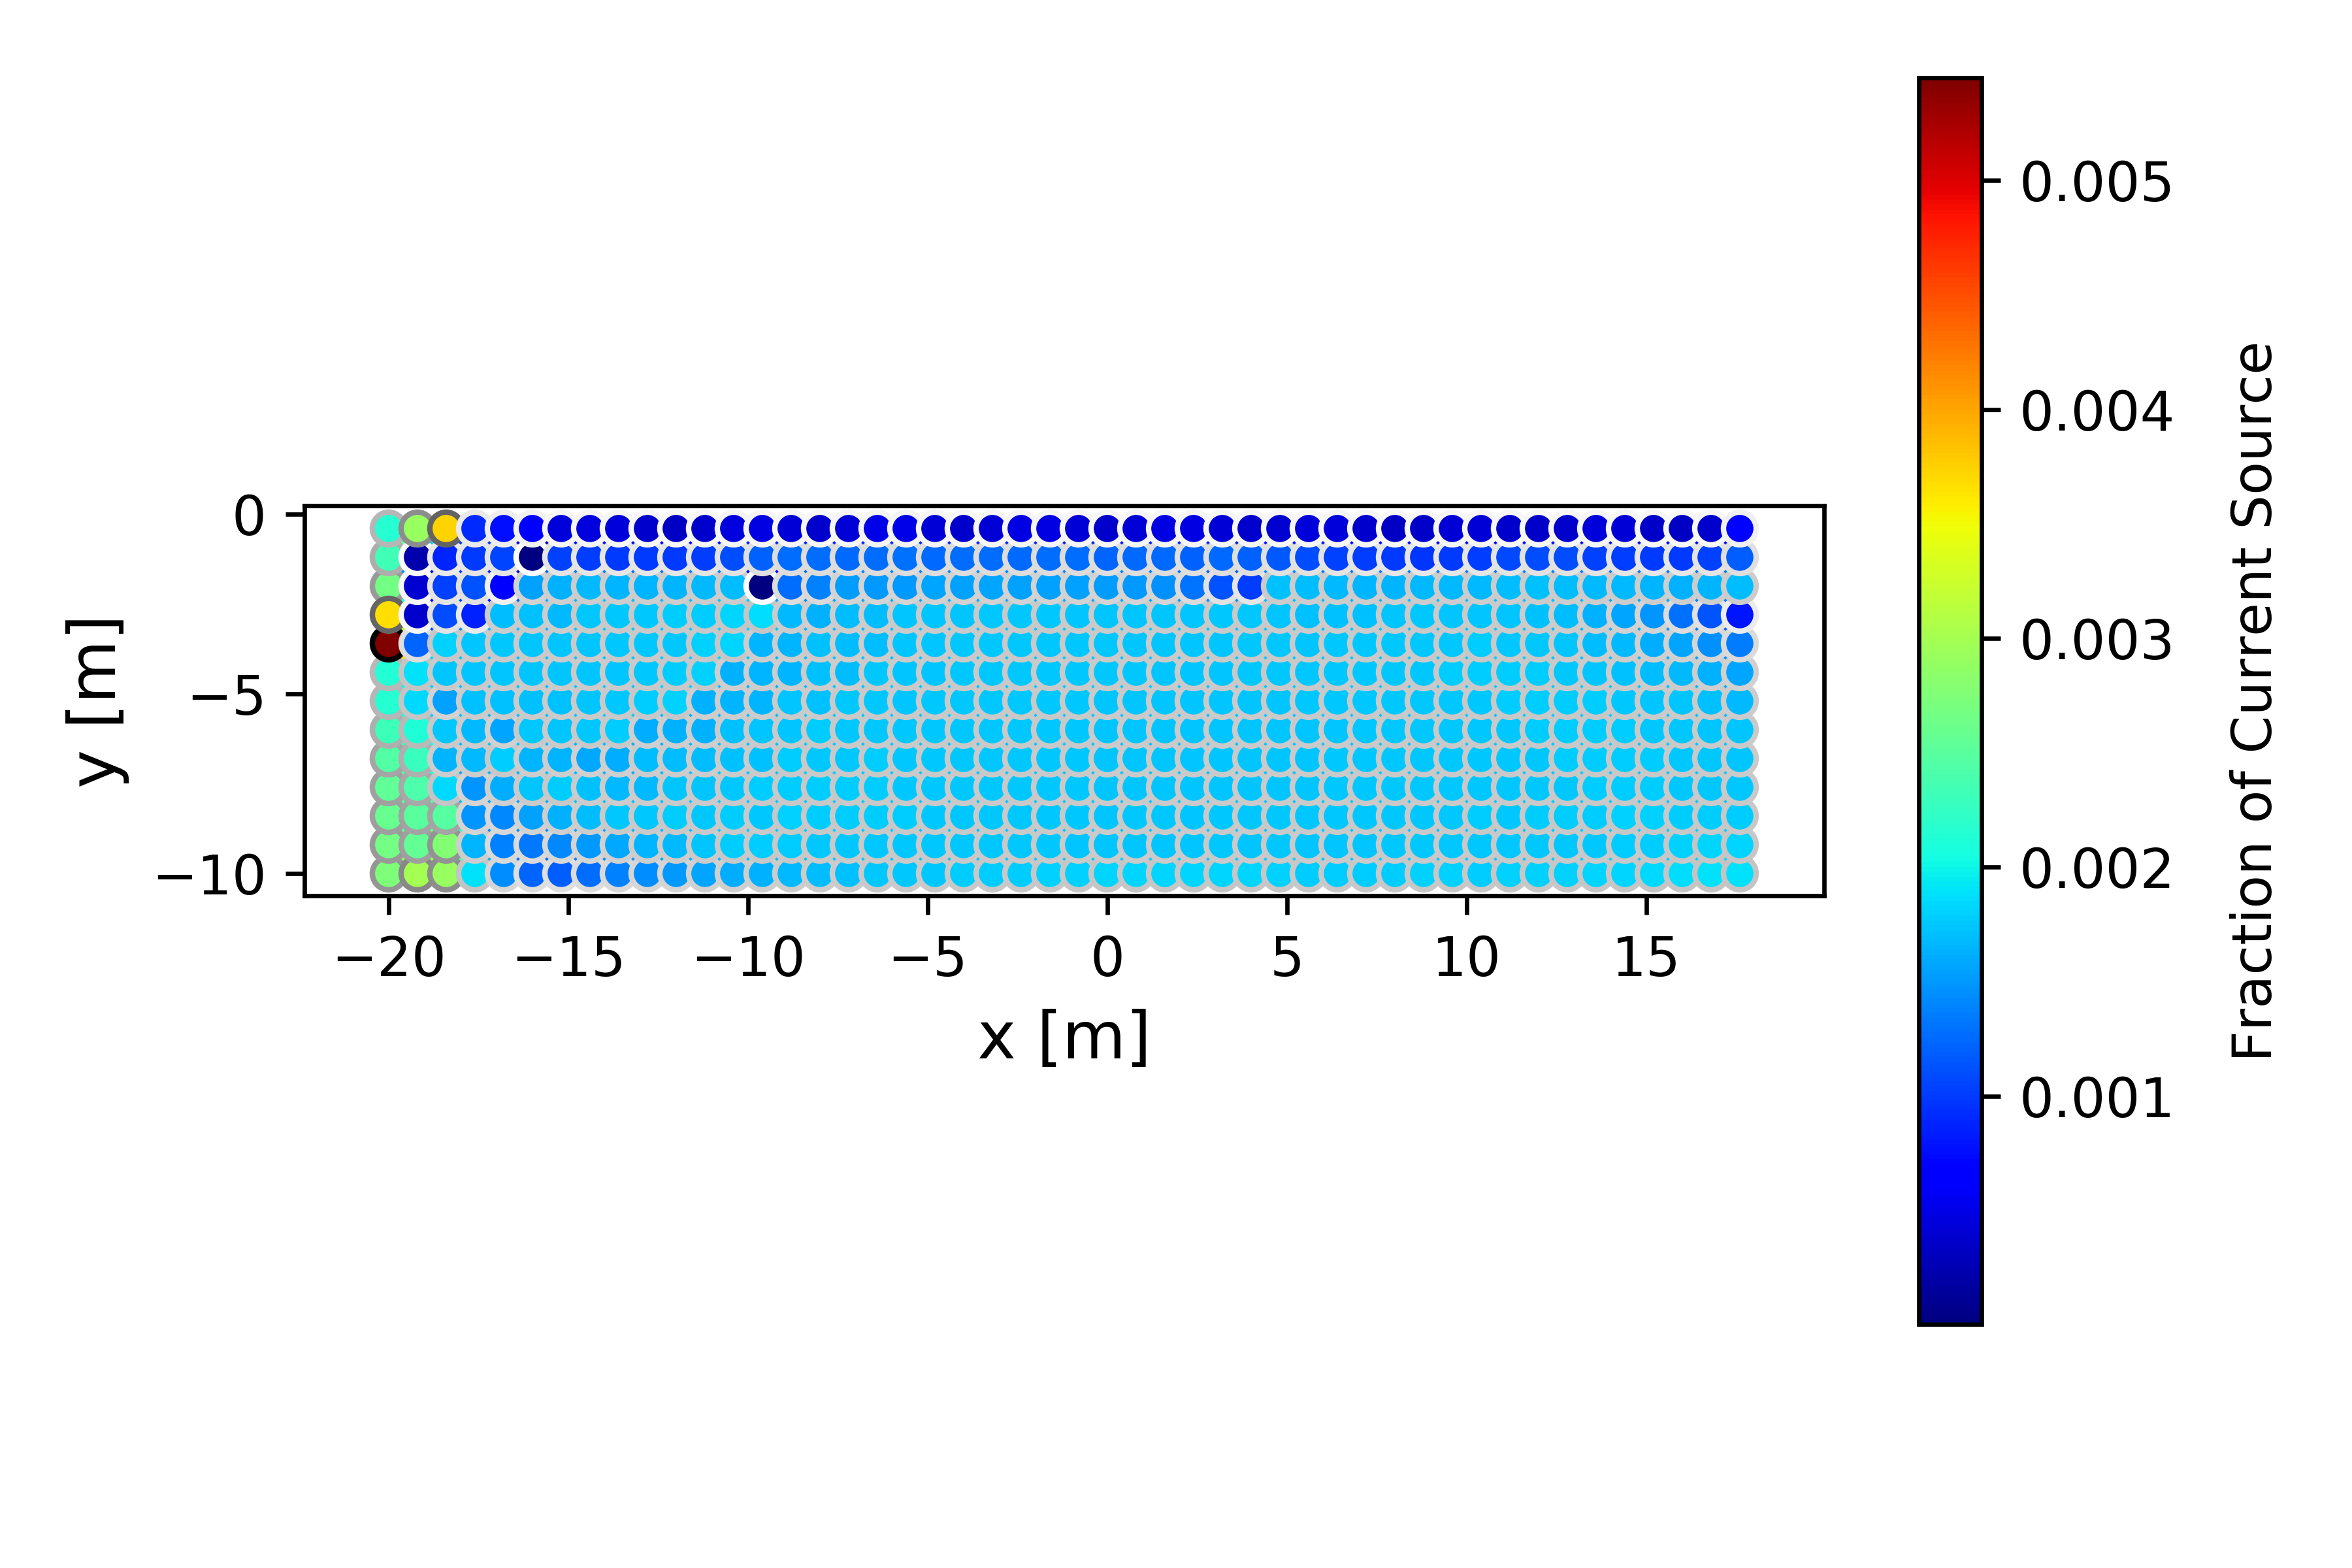
\includegraphics[width=8cm]{iCSD.png}}
	\subcaptionbox{Comparison between laboratory and simulated MALM resistances. The simulation of the resistances bases on the inverted resistivity distribution (BERT) and estimated current source distribution.\label{MALMcheck}}{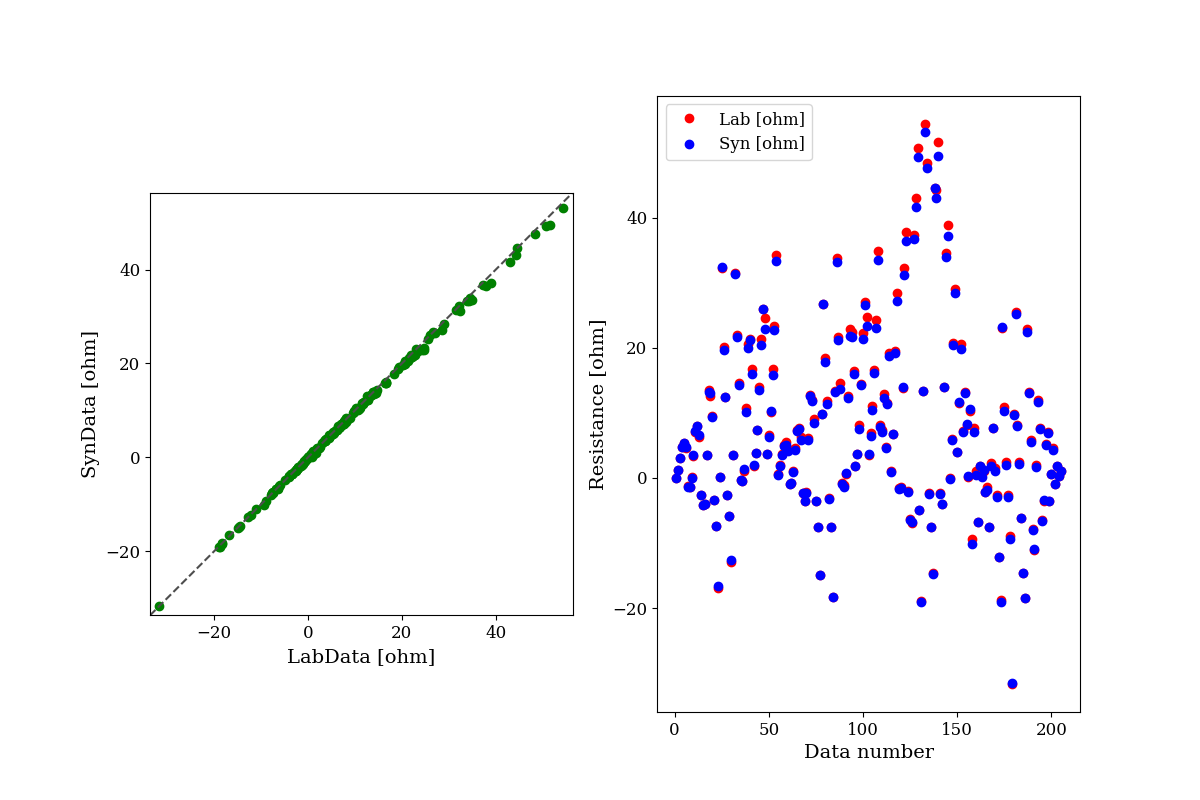
\includegraphics[width=8.5cm]{CheckPEST.png}}
	\caption{Lab experiment with single source.\label{LabExperiment}}
\end{figure}
\clearpage

In order to test the overall resolution of the current source density inversion we performed 6 laboratory tests in which two point sources where placed at different distances. We could then verify if, and for which minimum distance, the two sources were correctly inverted. For this tests a non-homogeneous water conductivity was forced by the addition of salt, the values of resistivity agreed with the solution conductivity values measured with a conductivity meter. Furthermore, the overall current source density inversion appears to properly take into account the conductivity distribution.

\begin{figure*}[h]
	\centering
	\captionsetup[sub]{margin=0.4cm}
	\subcaptionbox{Inverted resistivity distribution.\label{ertwater2s}}{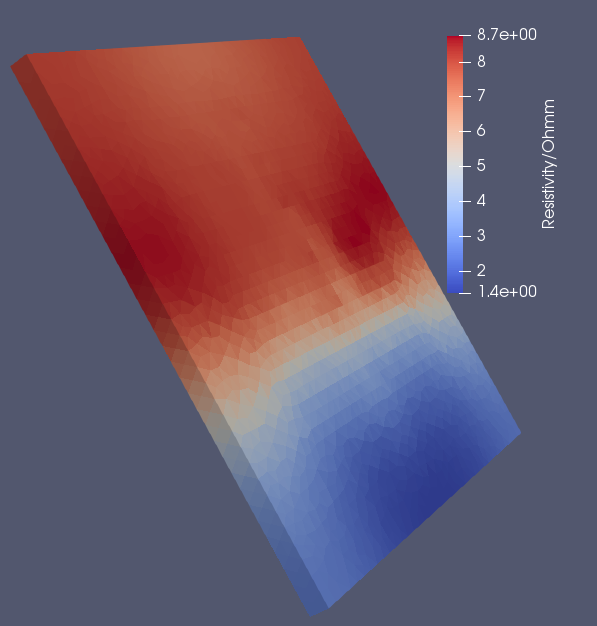
\includegraphics[width=8.2cm]{ertwater2s.png}}
	\subcaptionbox{Two current sources, experiment 4.\label{w2s4}}{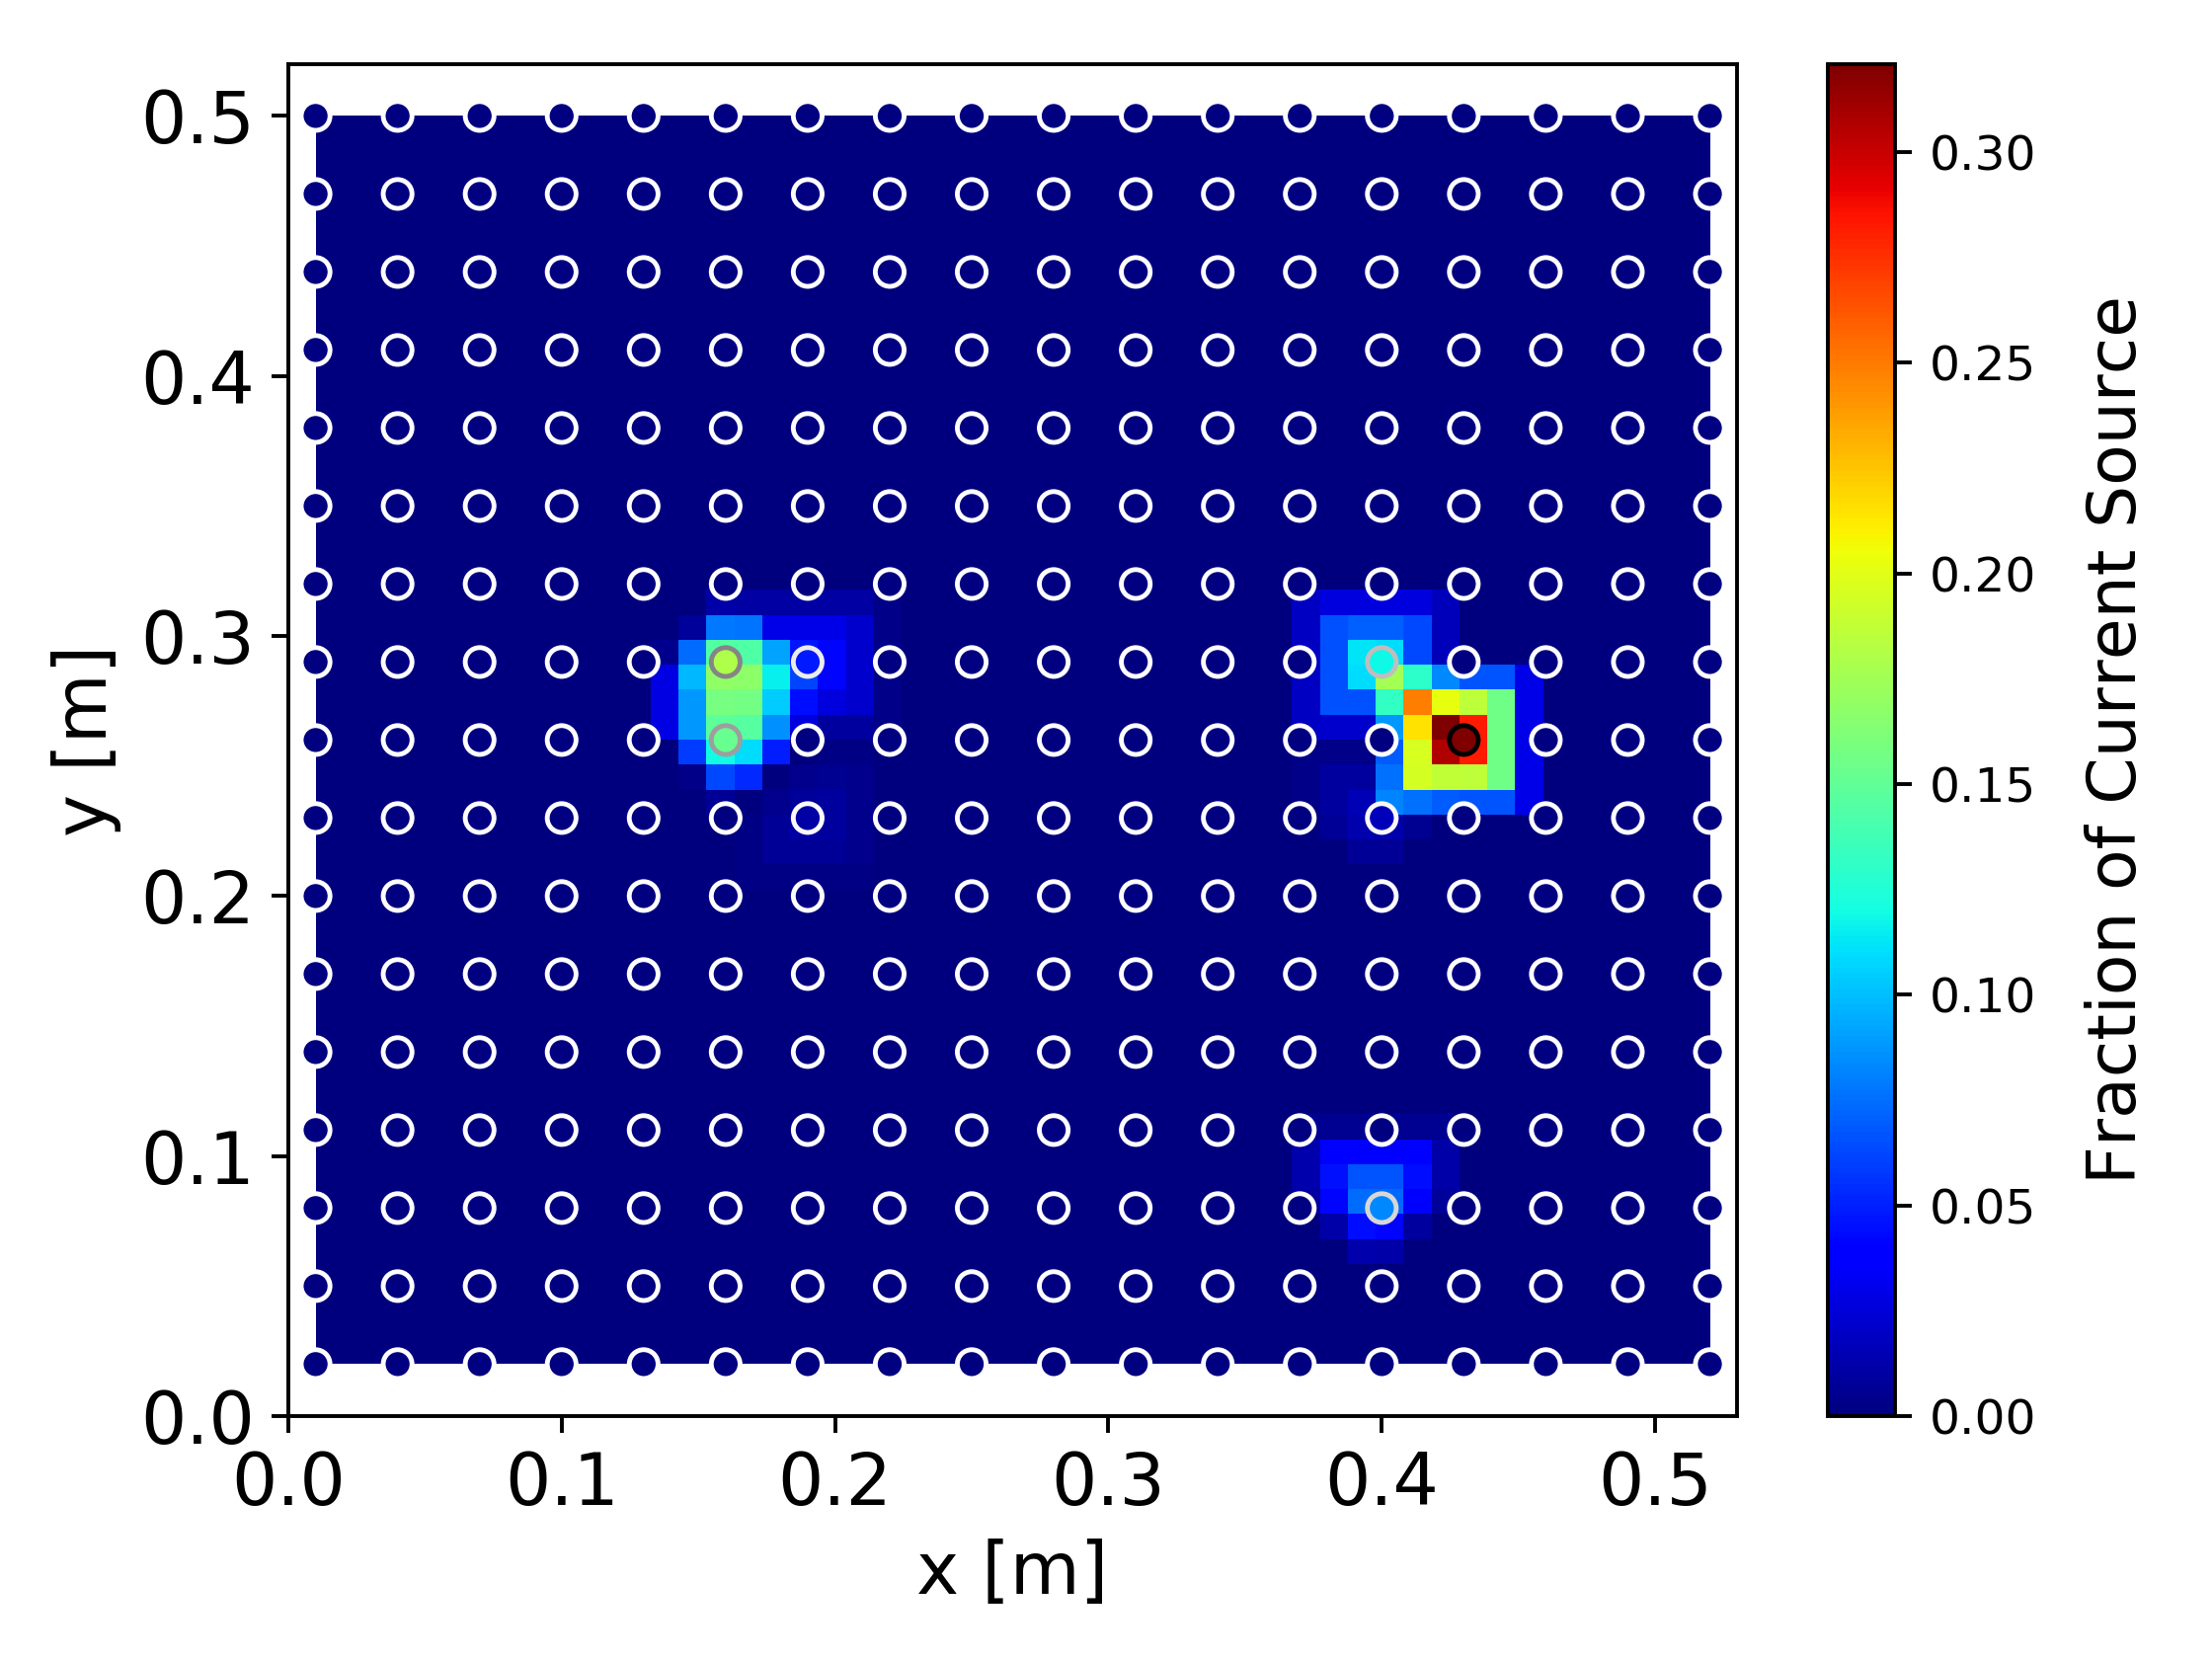
\includegraphics[width=8.2cm]{iCSDw4.png}}
	\subcaptionbox{Two current sources, experiment 5.\label{w2s5}}{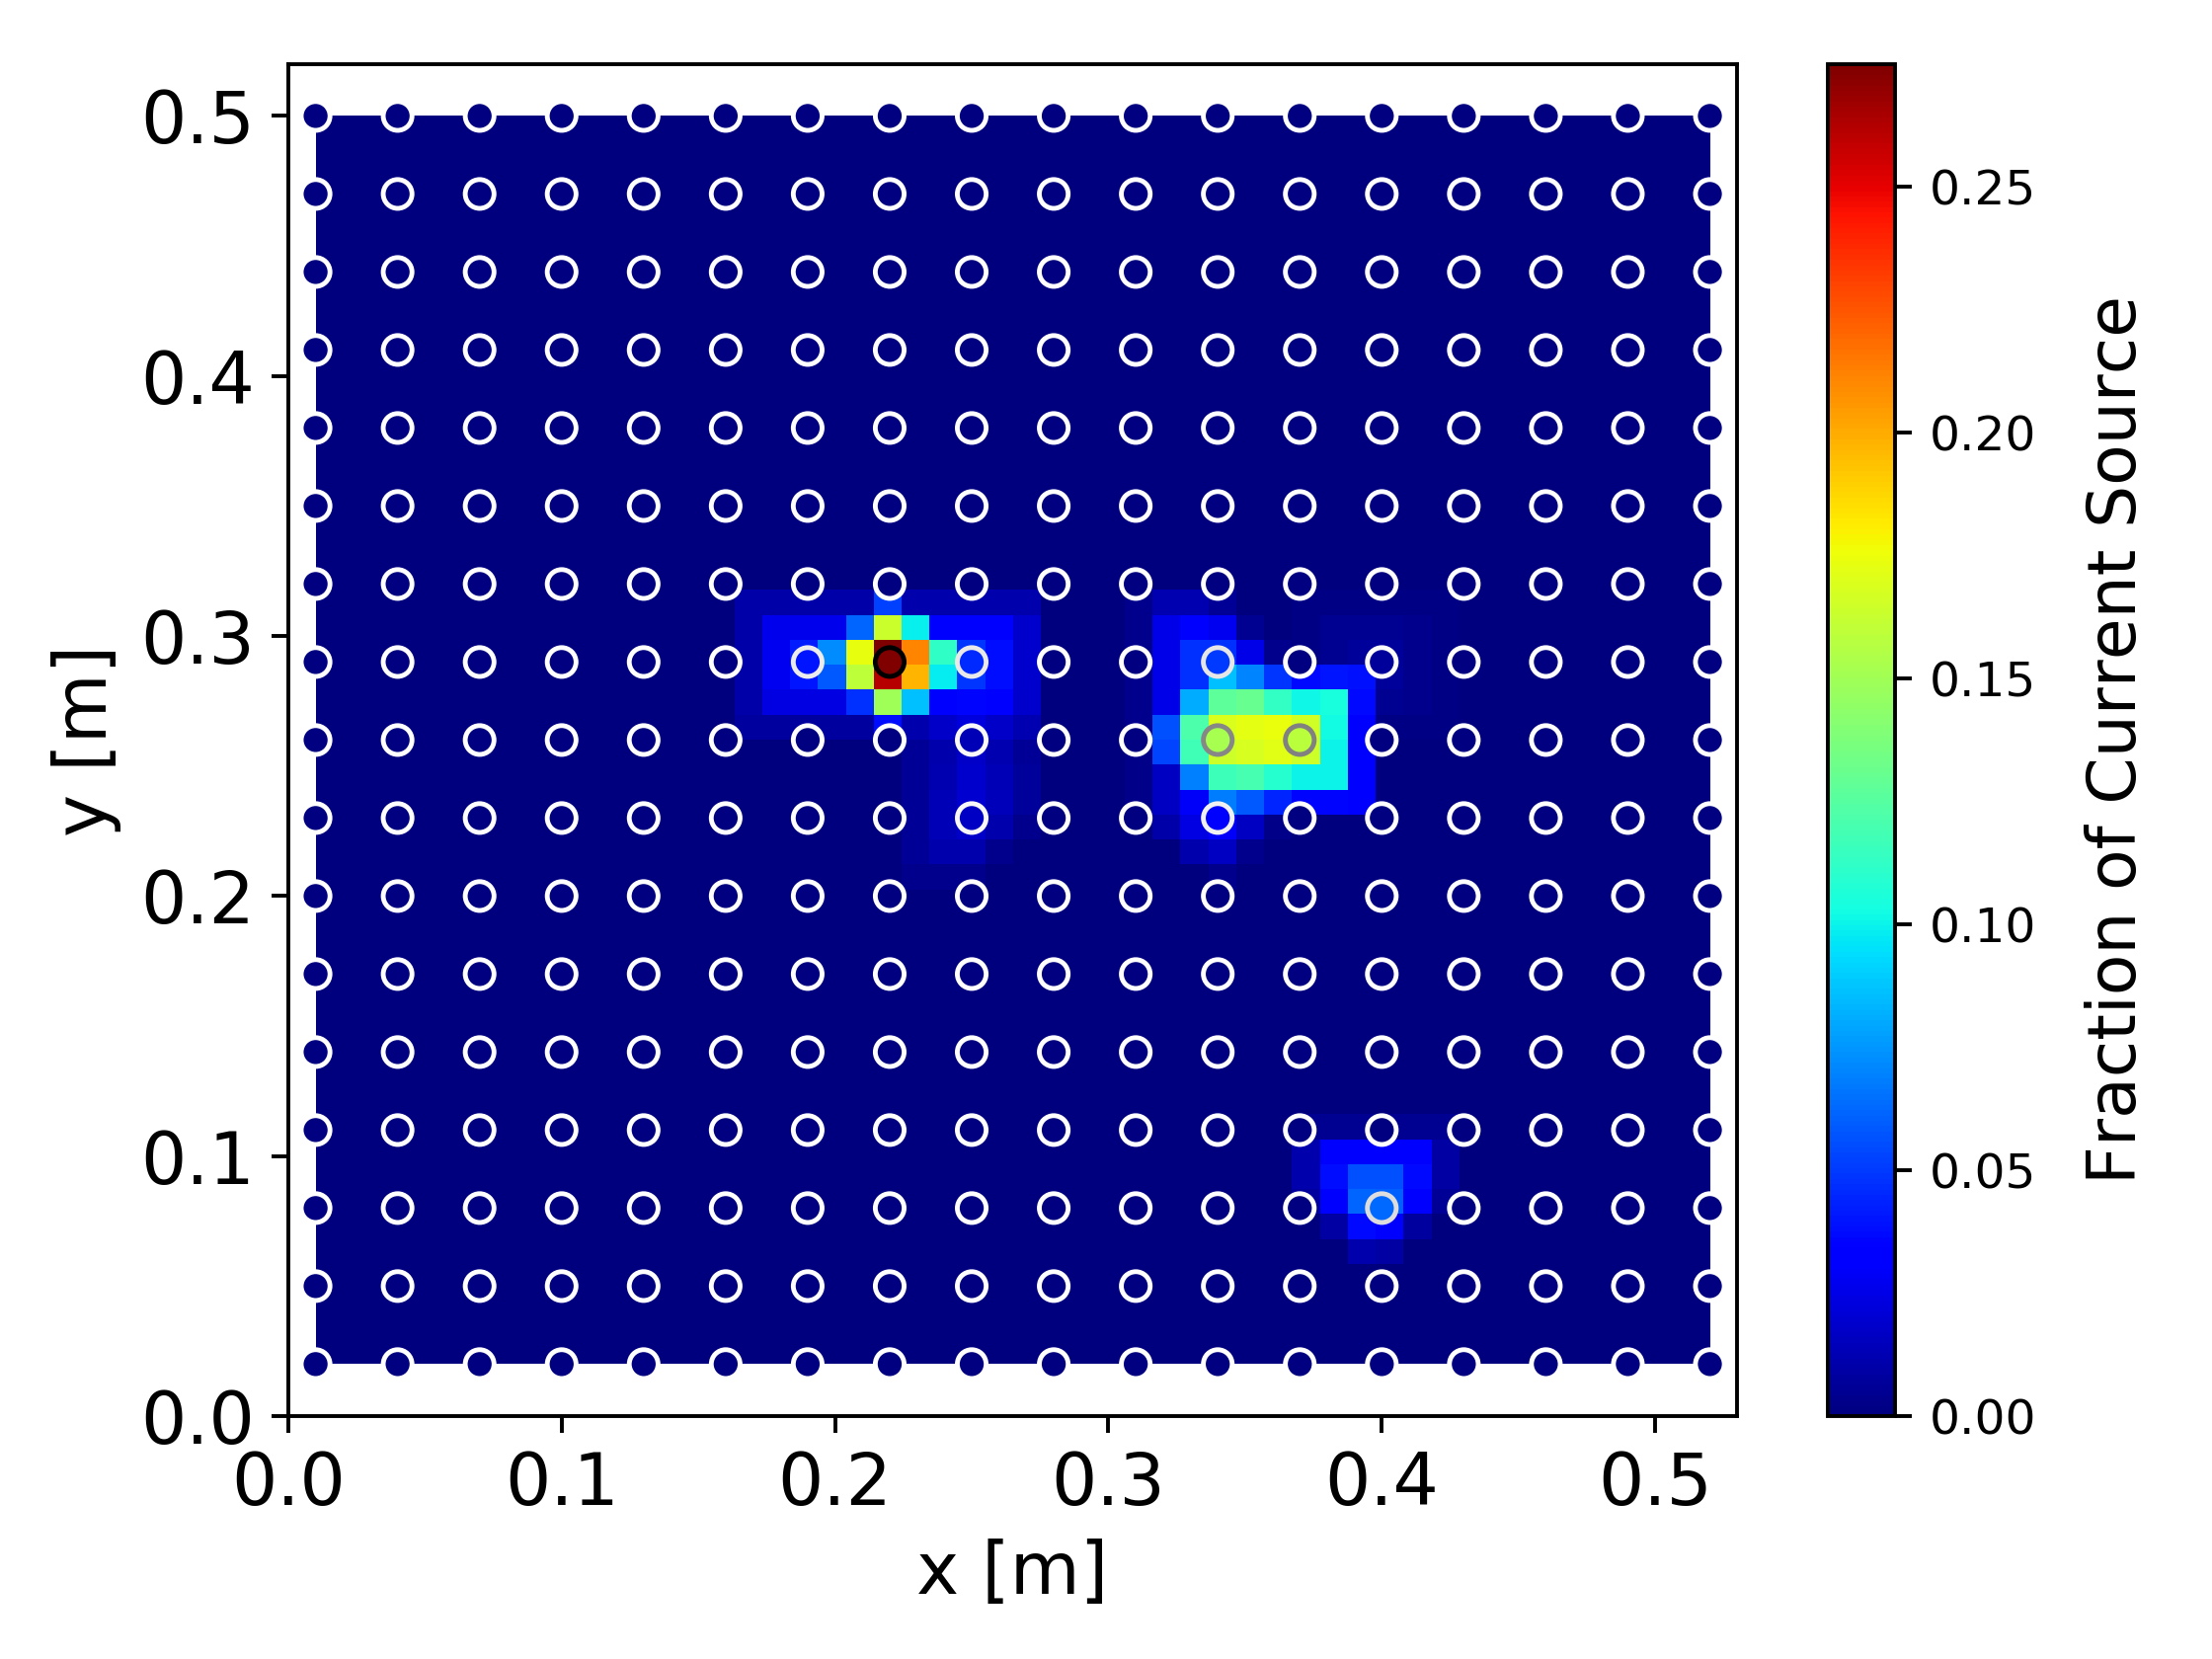
\includegraphics[width=8.2cm]{iCSDw5.png}}
	\subcaptionbox{Two current sources, experiment 6.\label{w2s6}}{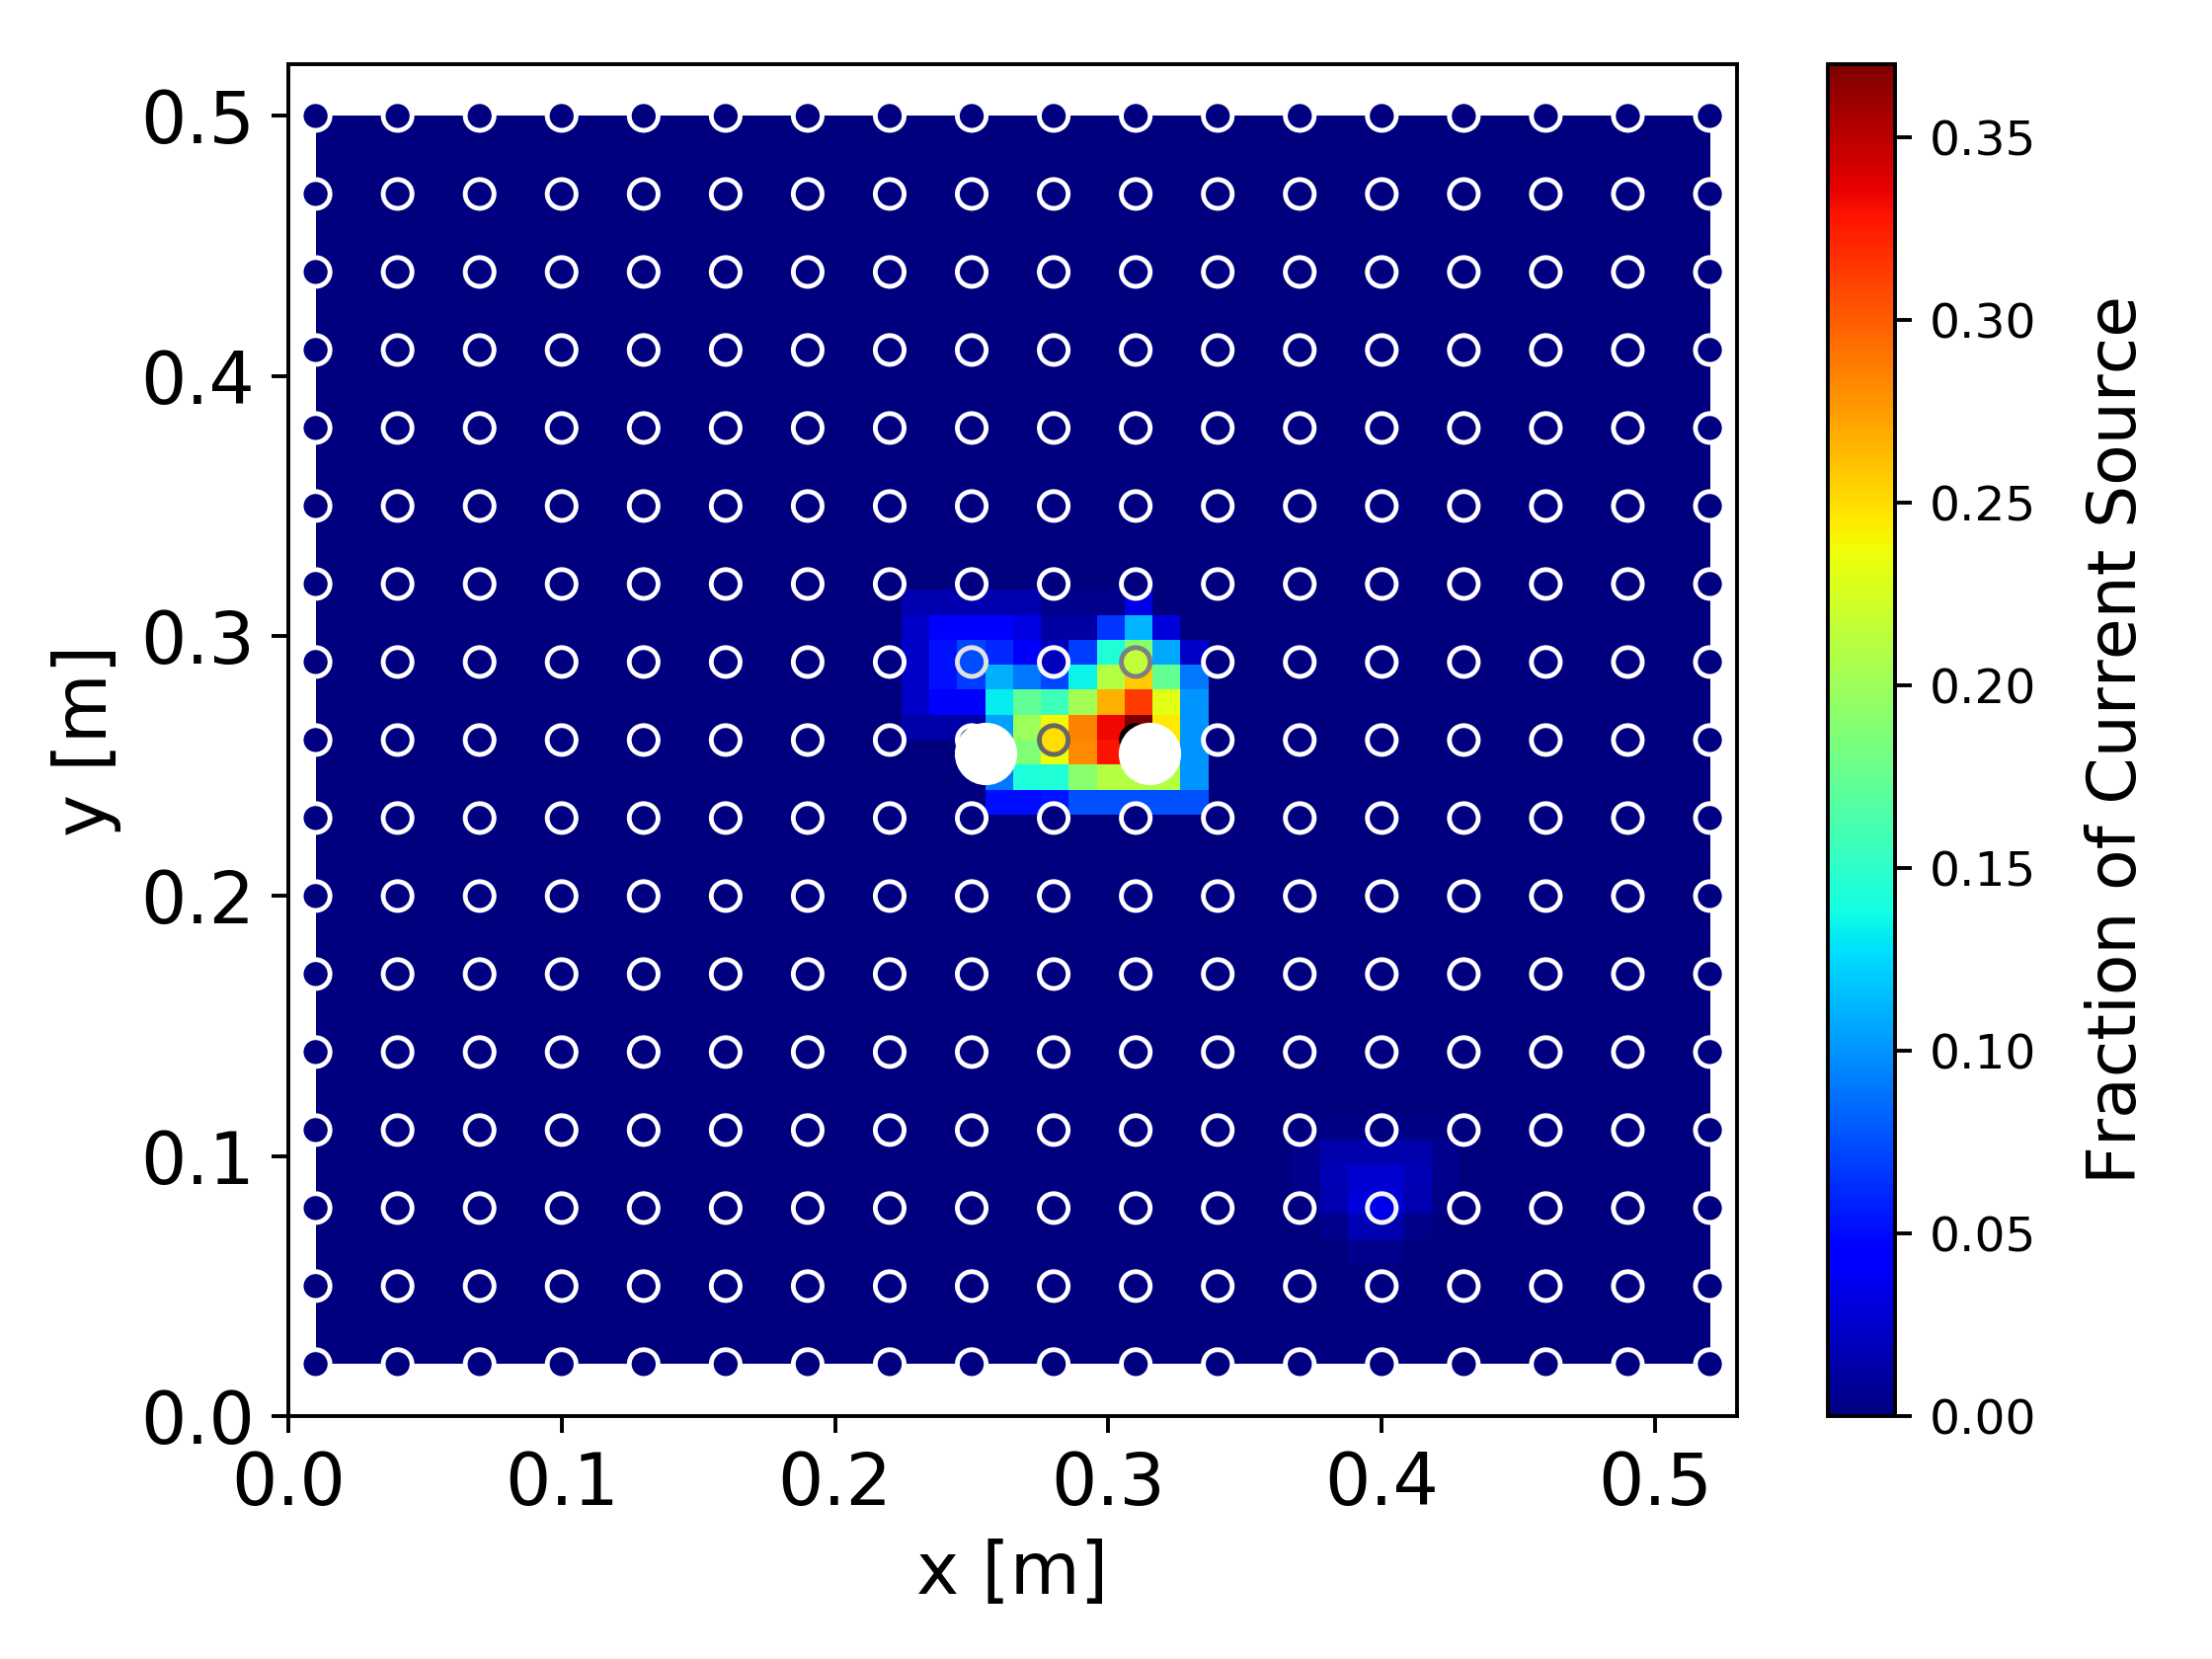
\includegraphics[width=8.5cm]{iCSDw6.png}}
	\caption{Lab experiment with two sources, the sources are correctly located and distinguished in experiments 4 and 5. In experiment 6 the two sources are not distinguished, see white dots, and a unique elongated source results from the inversion process.\label{TwoSources}}
\end{figure*}

\section{Plant in water}

After the numerical and laboratory methodological tests, we moved to explore the current source densities associated with MALM measurements on maize plants. In two first experiments the roots we positioned in the a rhizotron filed with water.

\begin{figure}[p]
	\centering
	\captionsetup[sub]{margin=0.4cm}
	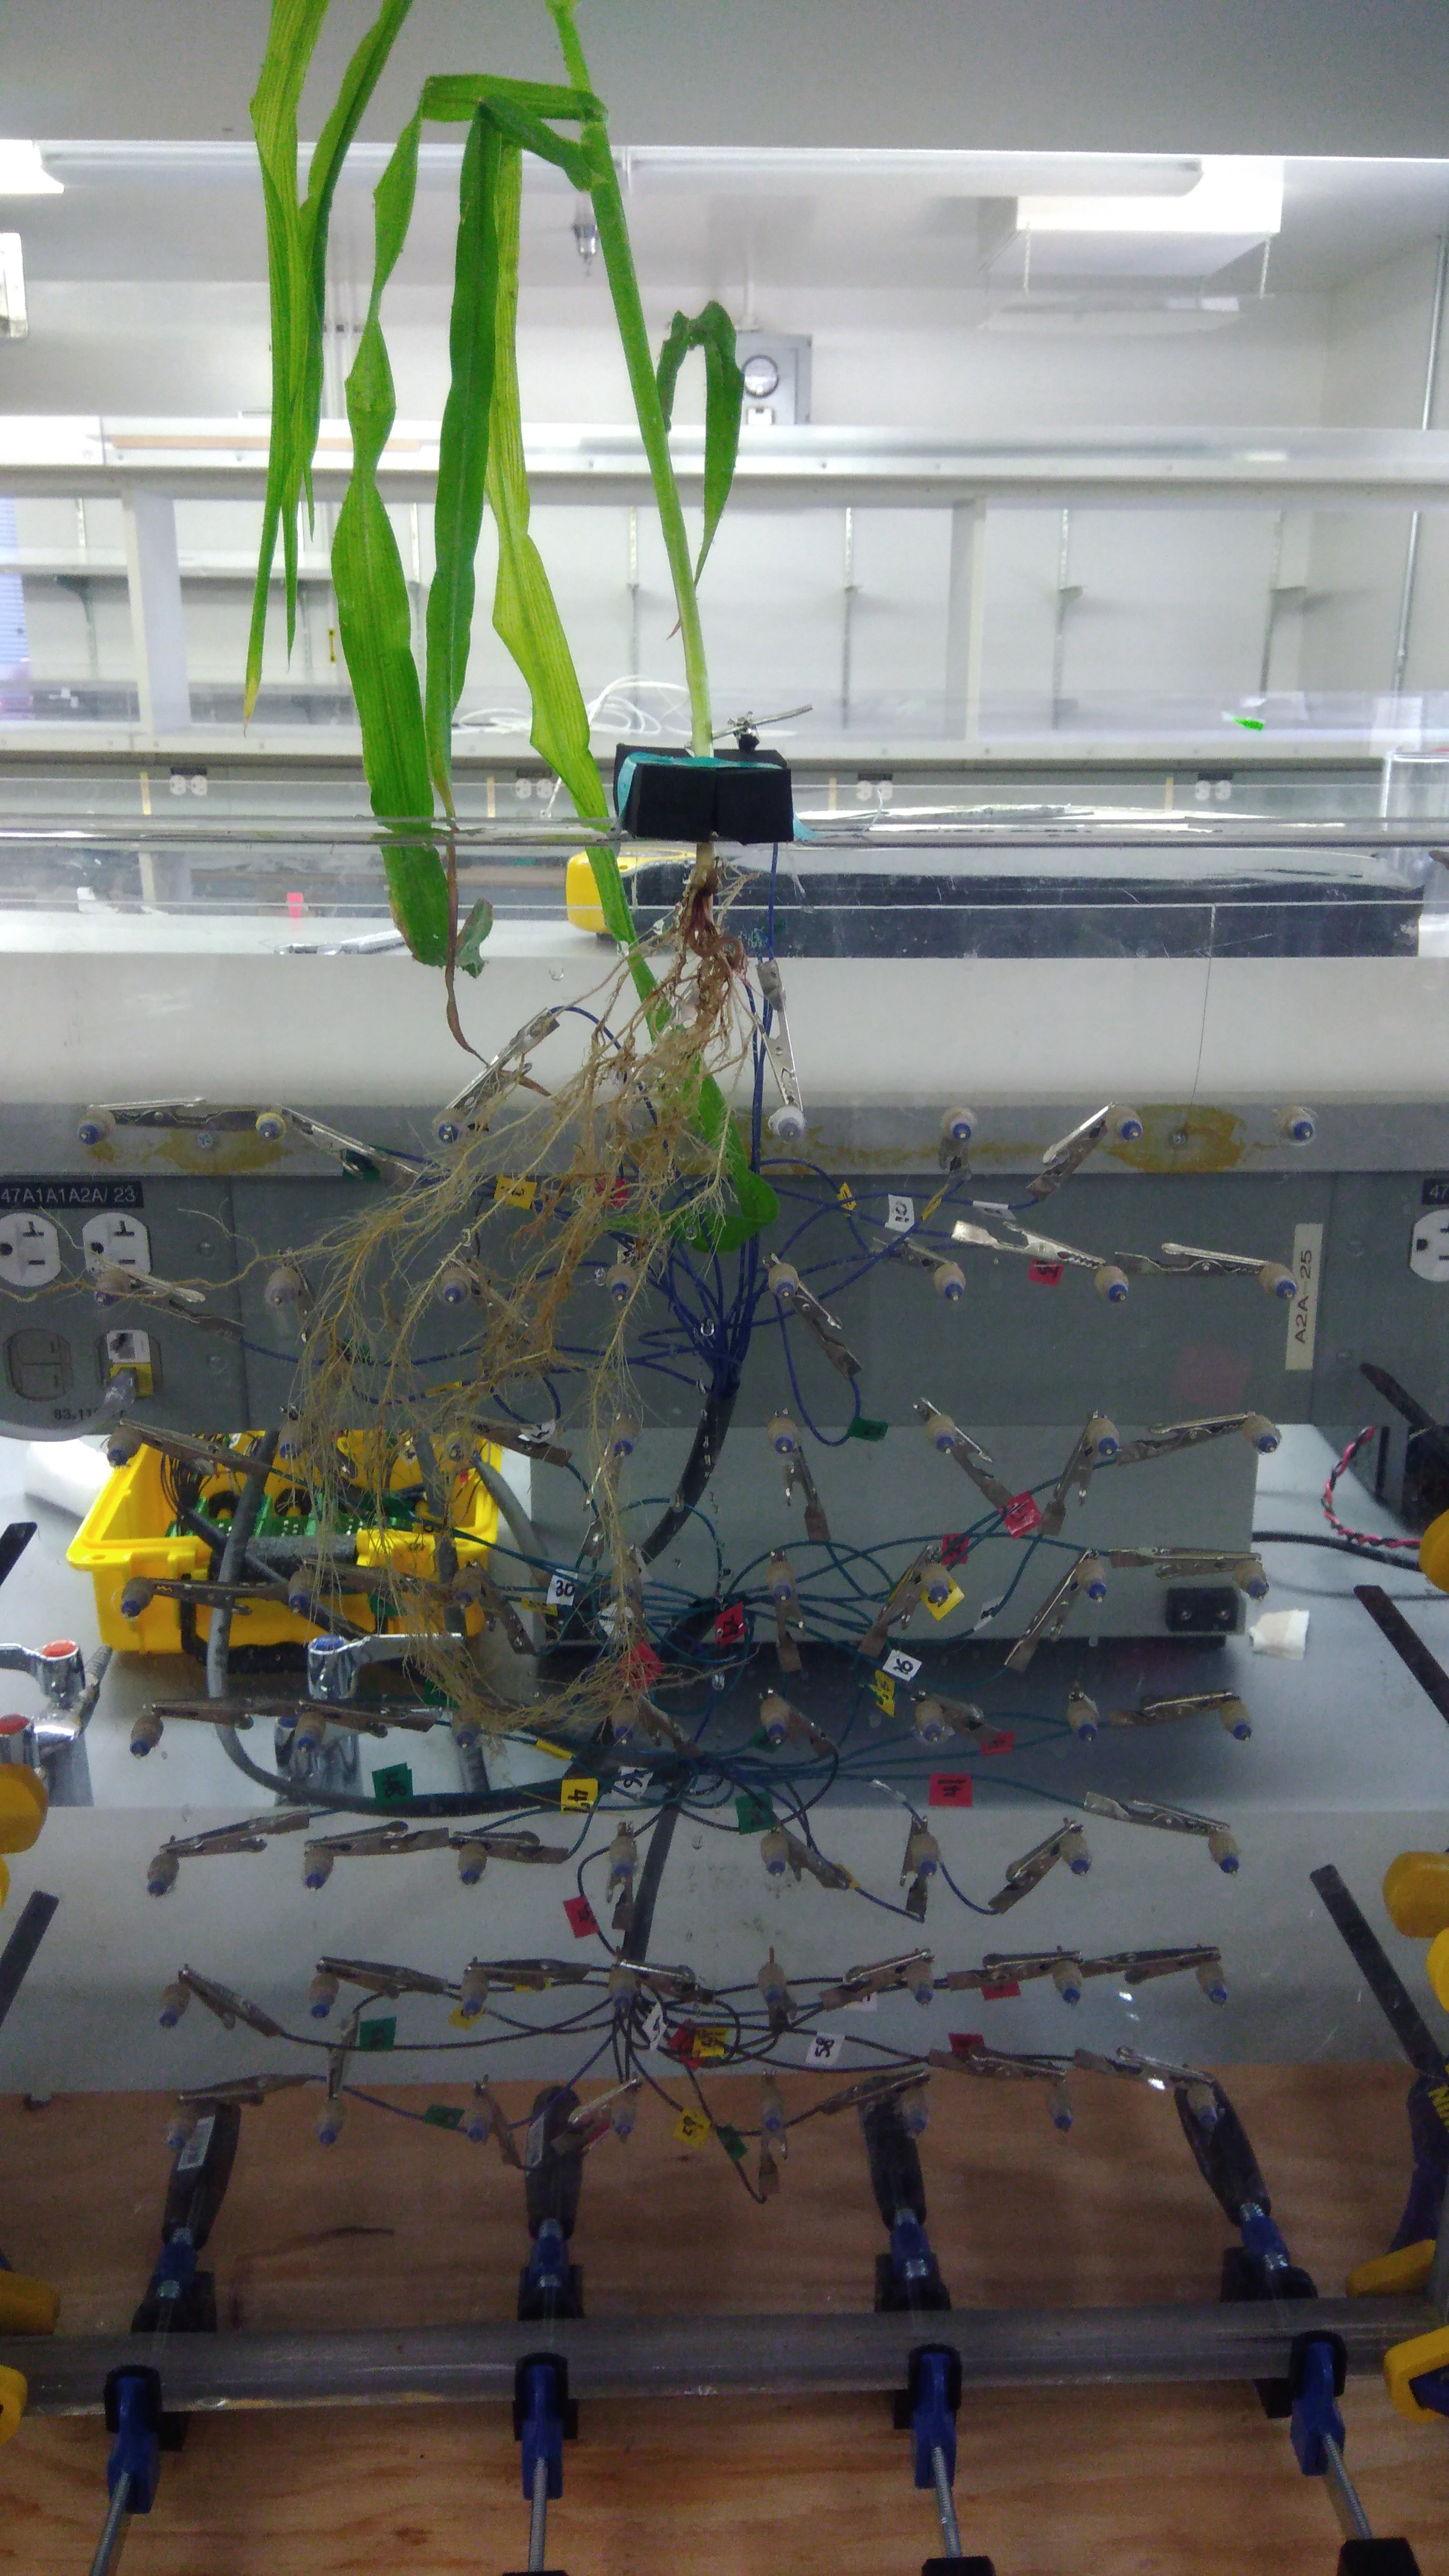
\includegraphics[width=8cm]{plant_malm_water.jpg}
	\caption{Plant experiment with water.\label{plant_water}}
\end{figure}

\begin{figure}[p]
	\centering
	\captionsetup[sub]{margin=0.4cm}
	\subcaptionbox{Plant 1.\label{WP1}}{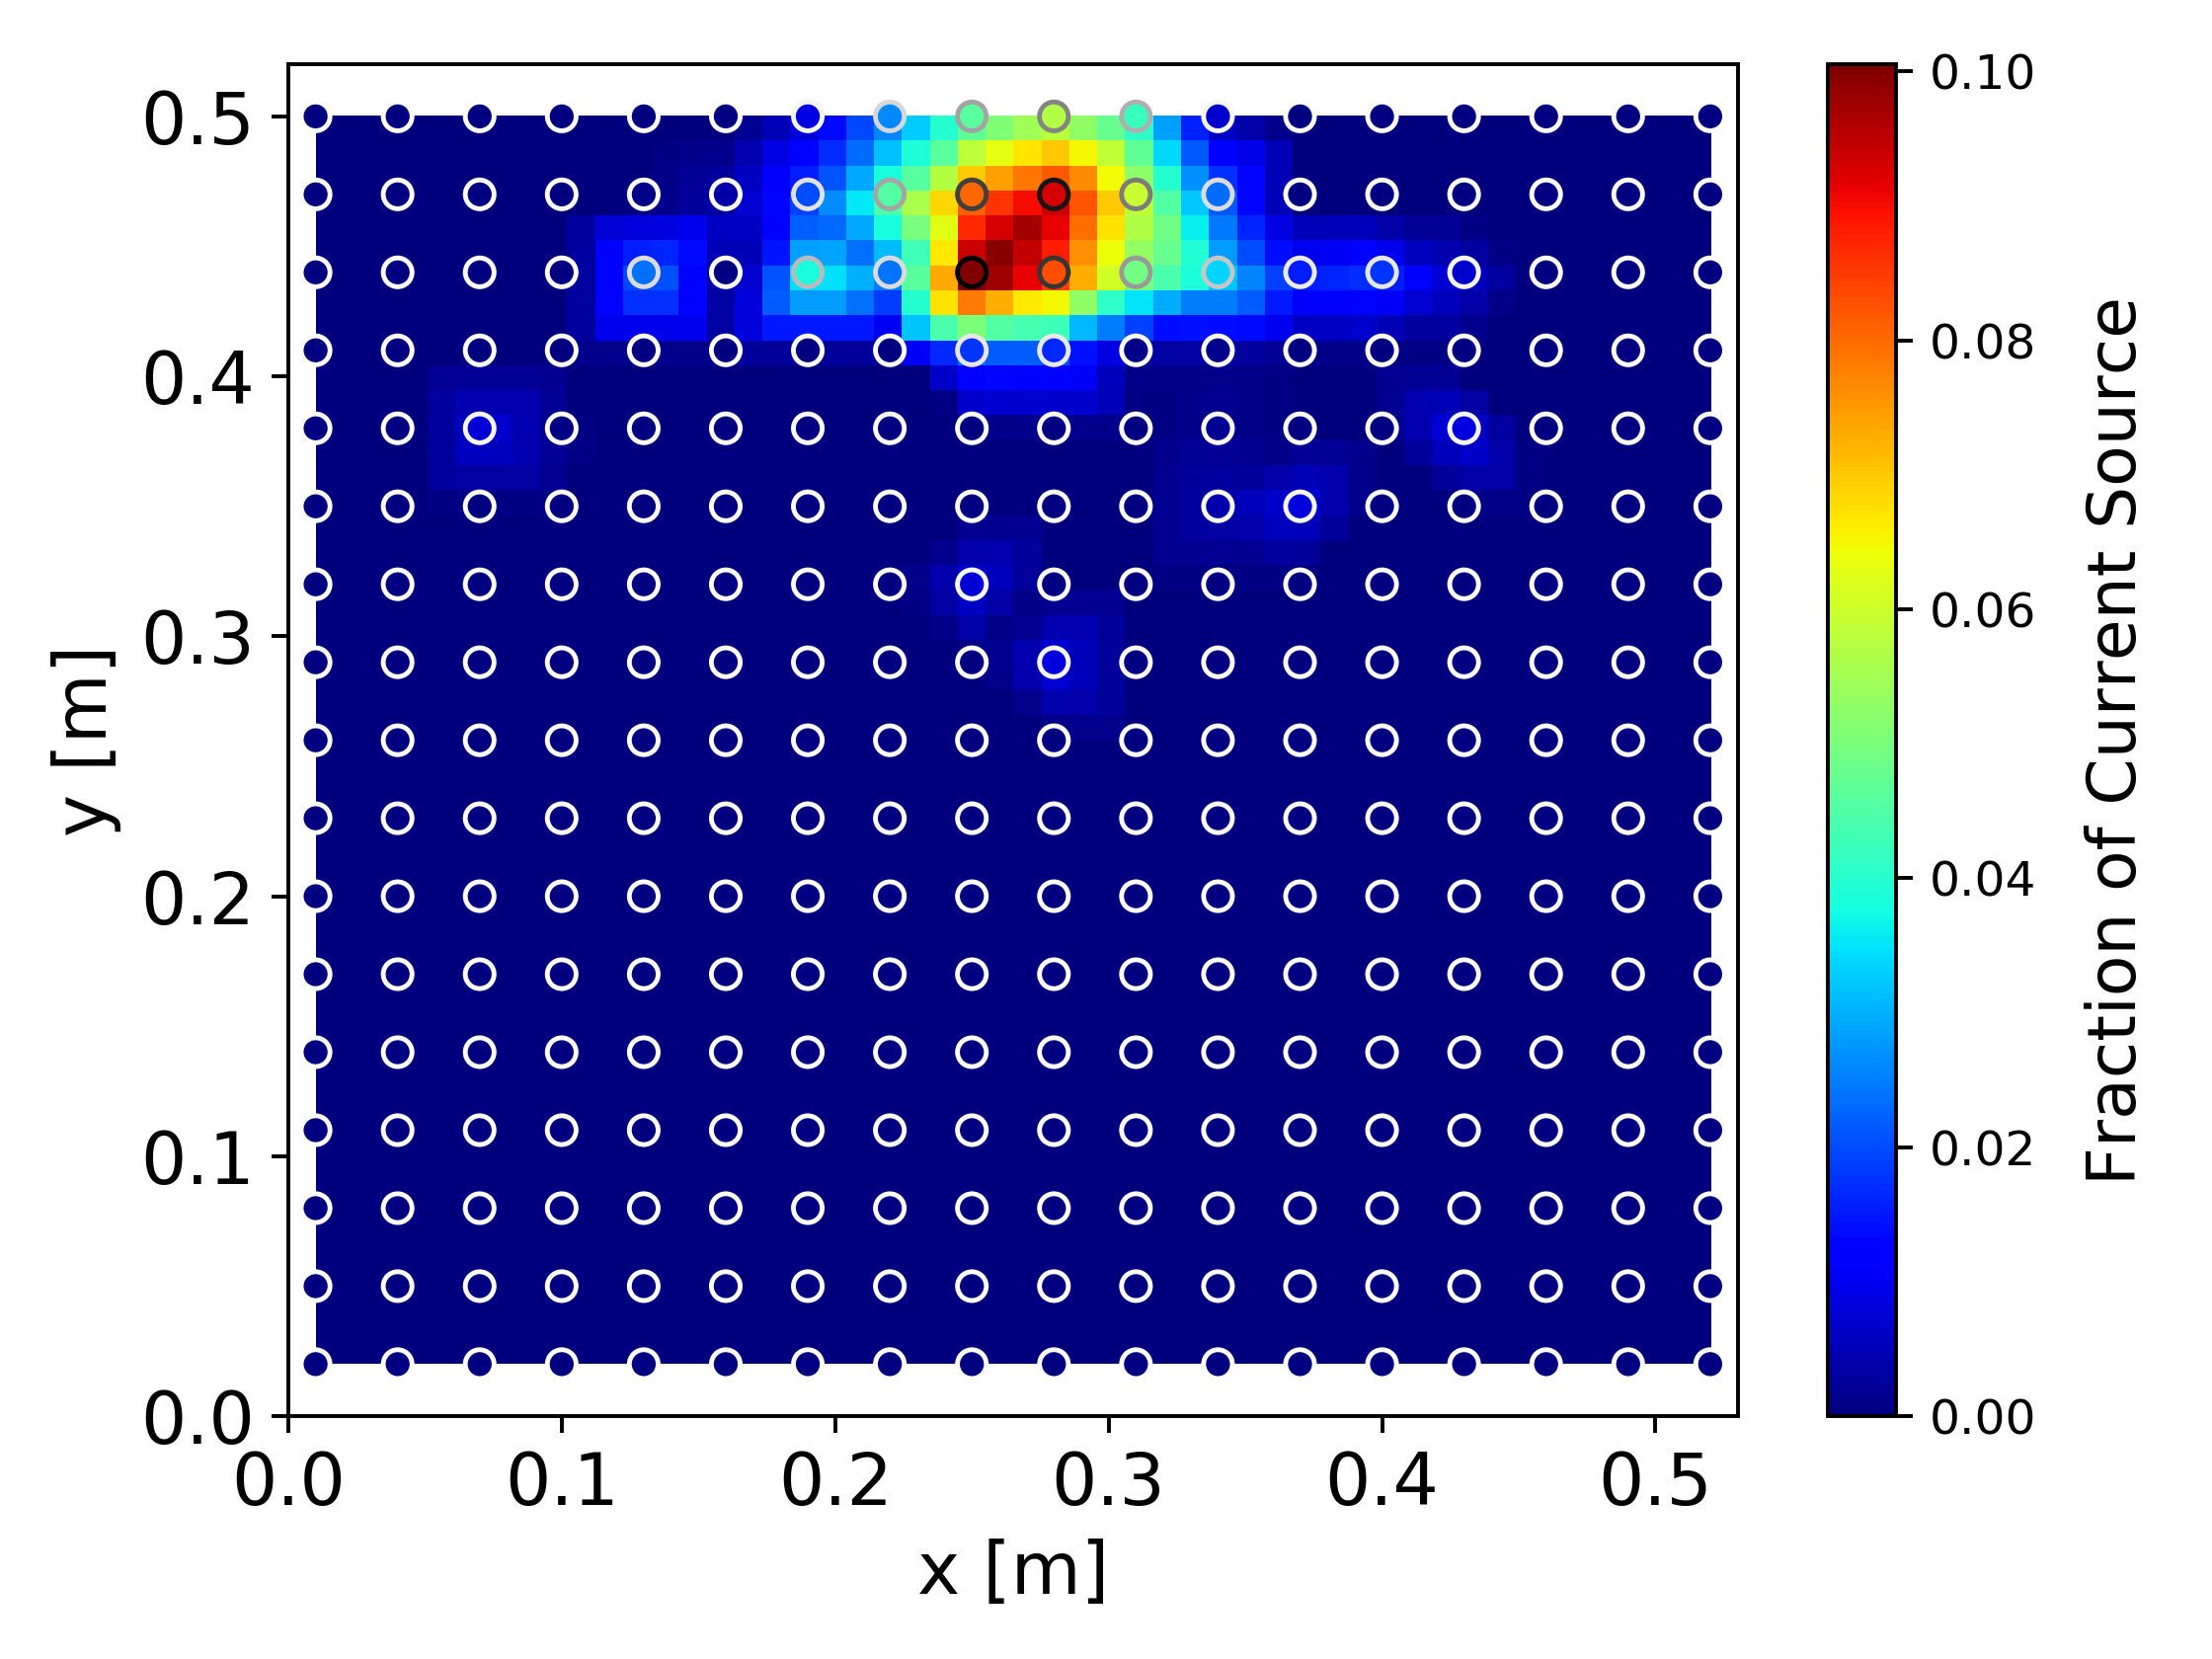
\includegraphics[width=8cm]{iCSDPlant1.png}}
	\subcaptionbox{Plant 2.\label{WP2}}{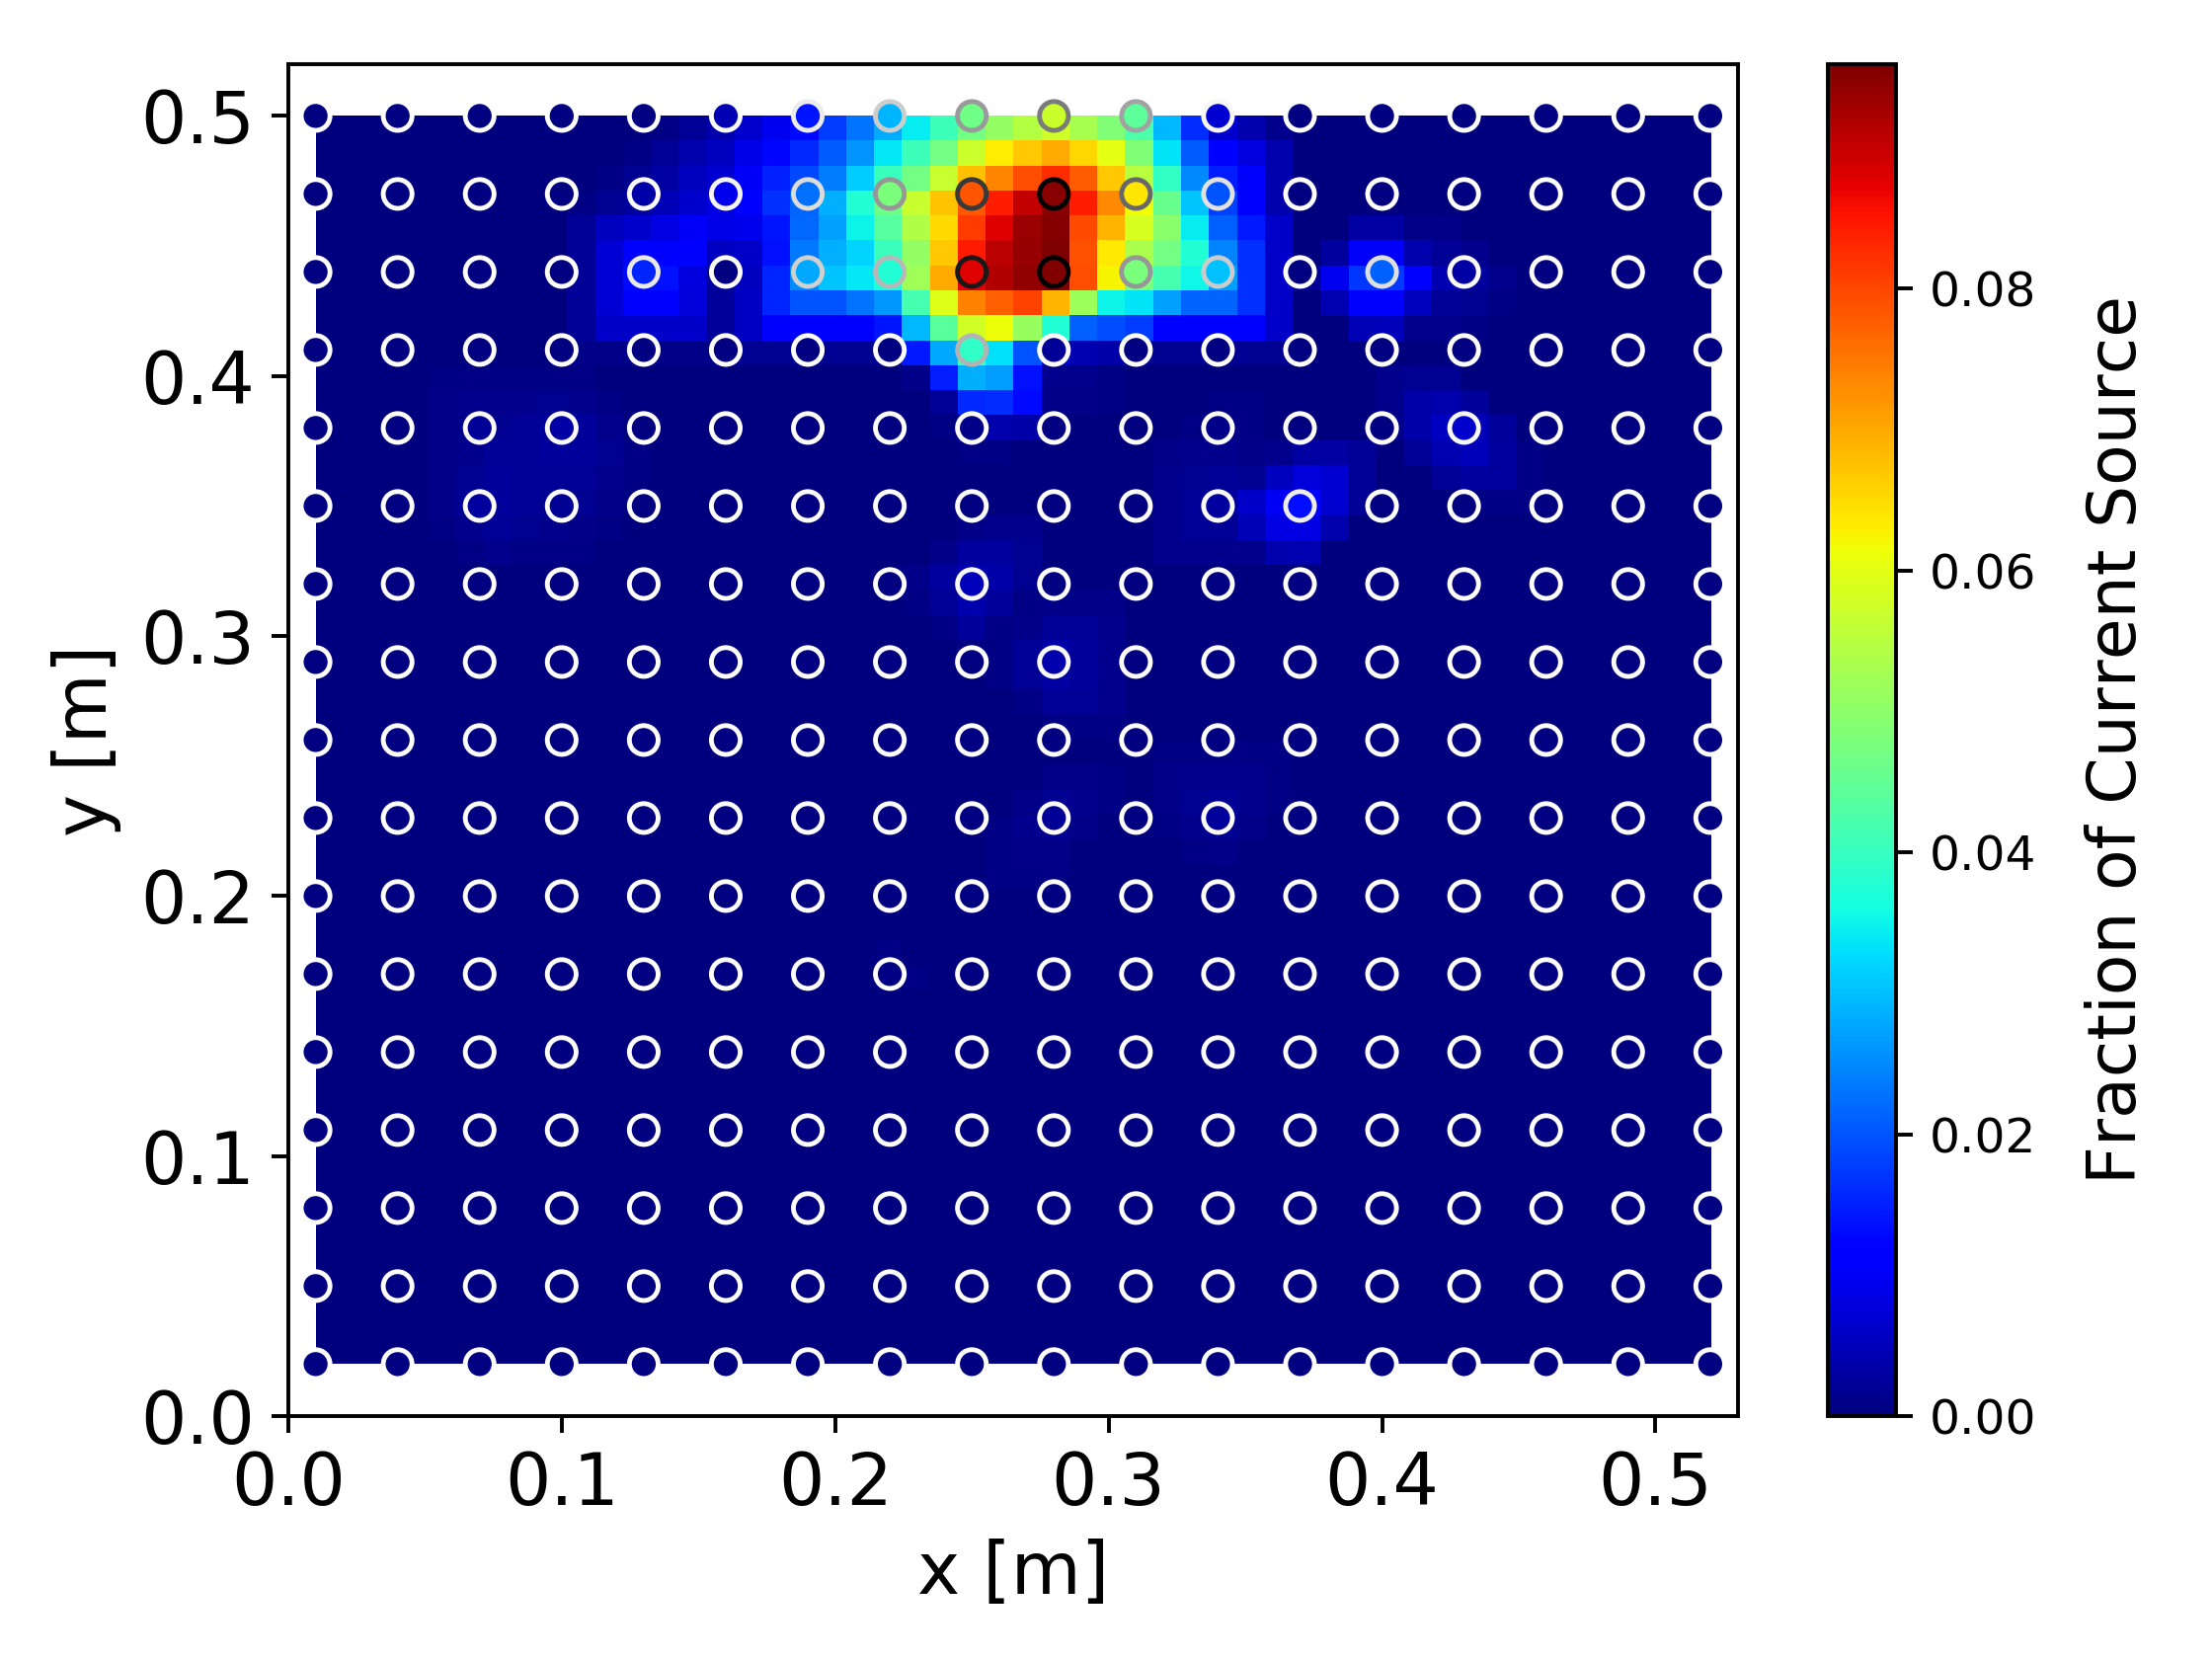
\includegraphics[width=8cm]{iCSDPlant2.png}}
	\caption{Current source densities obtained from the two laboratory experiments with maize plants in water.\label{iCSDWP}}
\end{figure}



\section{Plant in Soil}
On the basis of the positive initial tests, we performed an experiment with a maize plant in natural soil. An homogeneous distribution of the current source was used as initial value for the estimation procedure.
\vspace{2cm}
\begin{figure}[H]
	\centering
	\captionsetup[sub]{margin=0.4cm}
	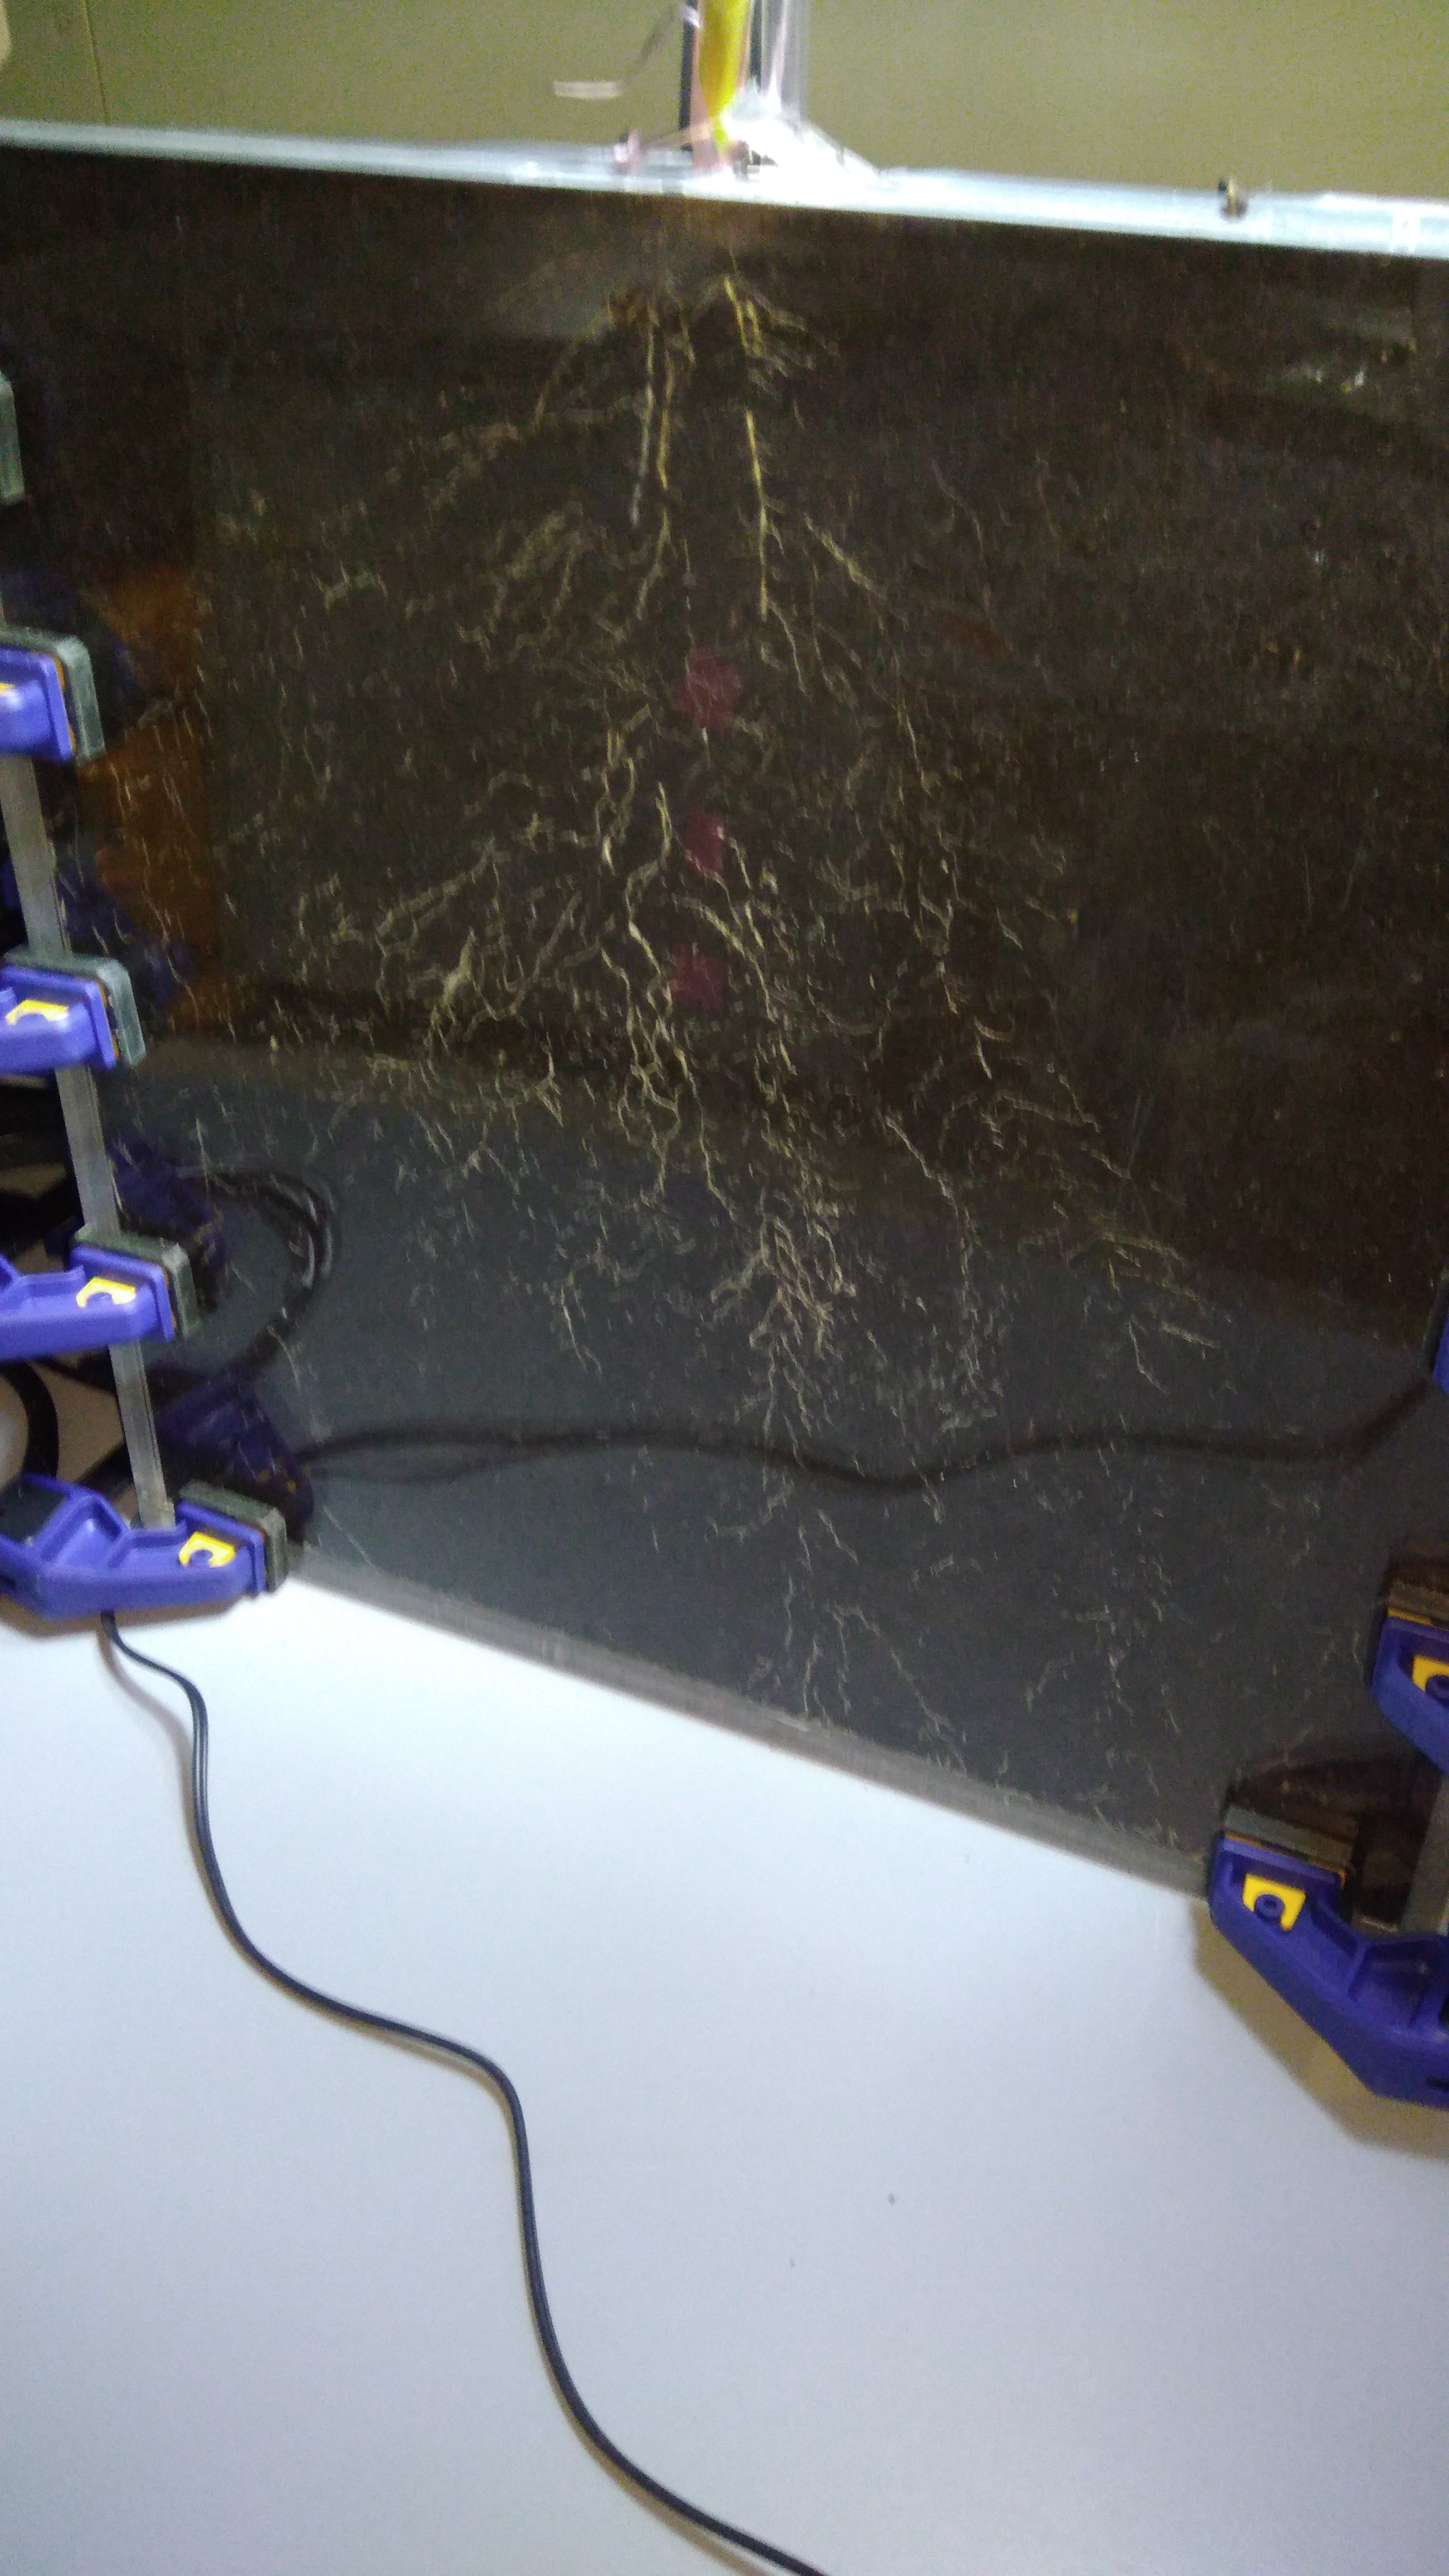
\includegraphics[width=8cm]{Plant.jpg}
	\caption{Distribution of the roots at the moment of the MALM acquisition.\label{Plant}}
\end{figure}

\begin{figure*}[p]
\centering
\captionsetup[sub]{margin=0.4cm}
\subcaptionbox{Inverted resistivity distribution.\label{PlantERT}}{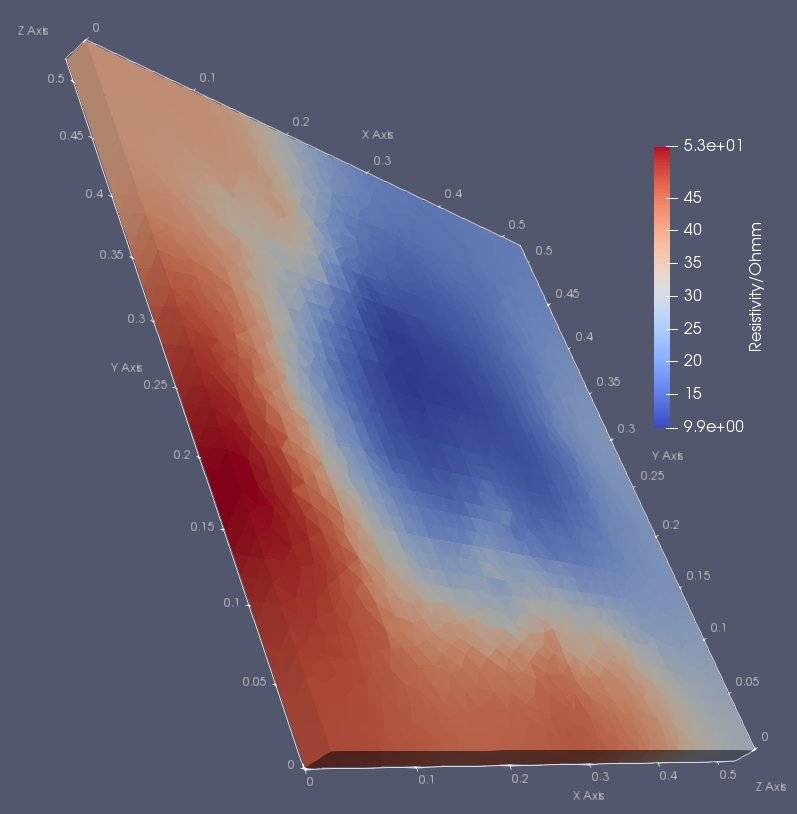
\includegraphics[width=8cm]{PlantERT.png}}
\subcaptionbox{ERT data check, comparison between laboratory ERT data and resistances modeled on the inverted resistivity model. The particular distribution of the misfit is likely due to the Occam regularization implemented by the ERT code. \label{PlantERTcheck}}{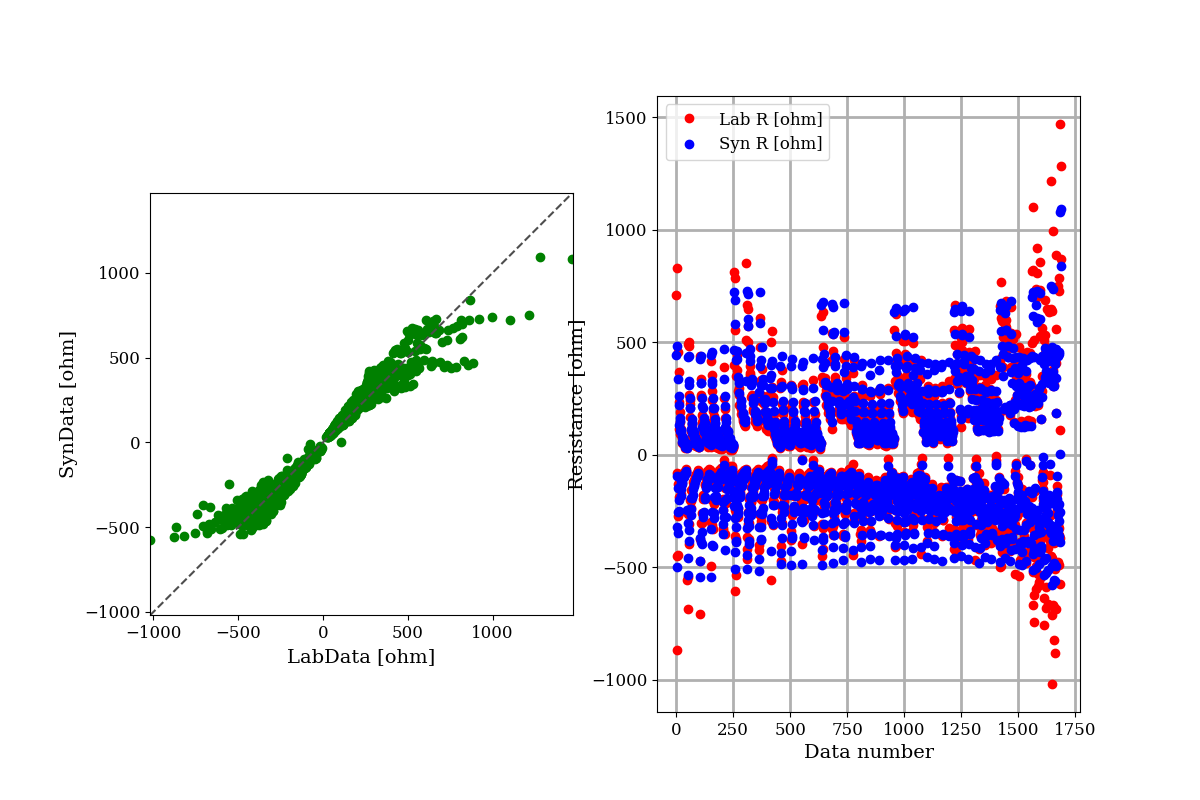
\includegraphics[width=8.5cm]{PlantERTCheck.png}}
\subcaptionbox{Estimated current source distribution, the red point represents the position of the return electrode.\label{PlantSCD}}{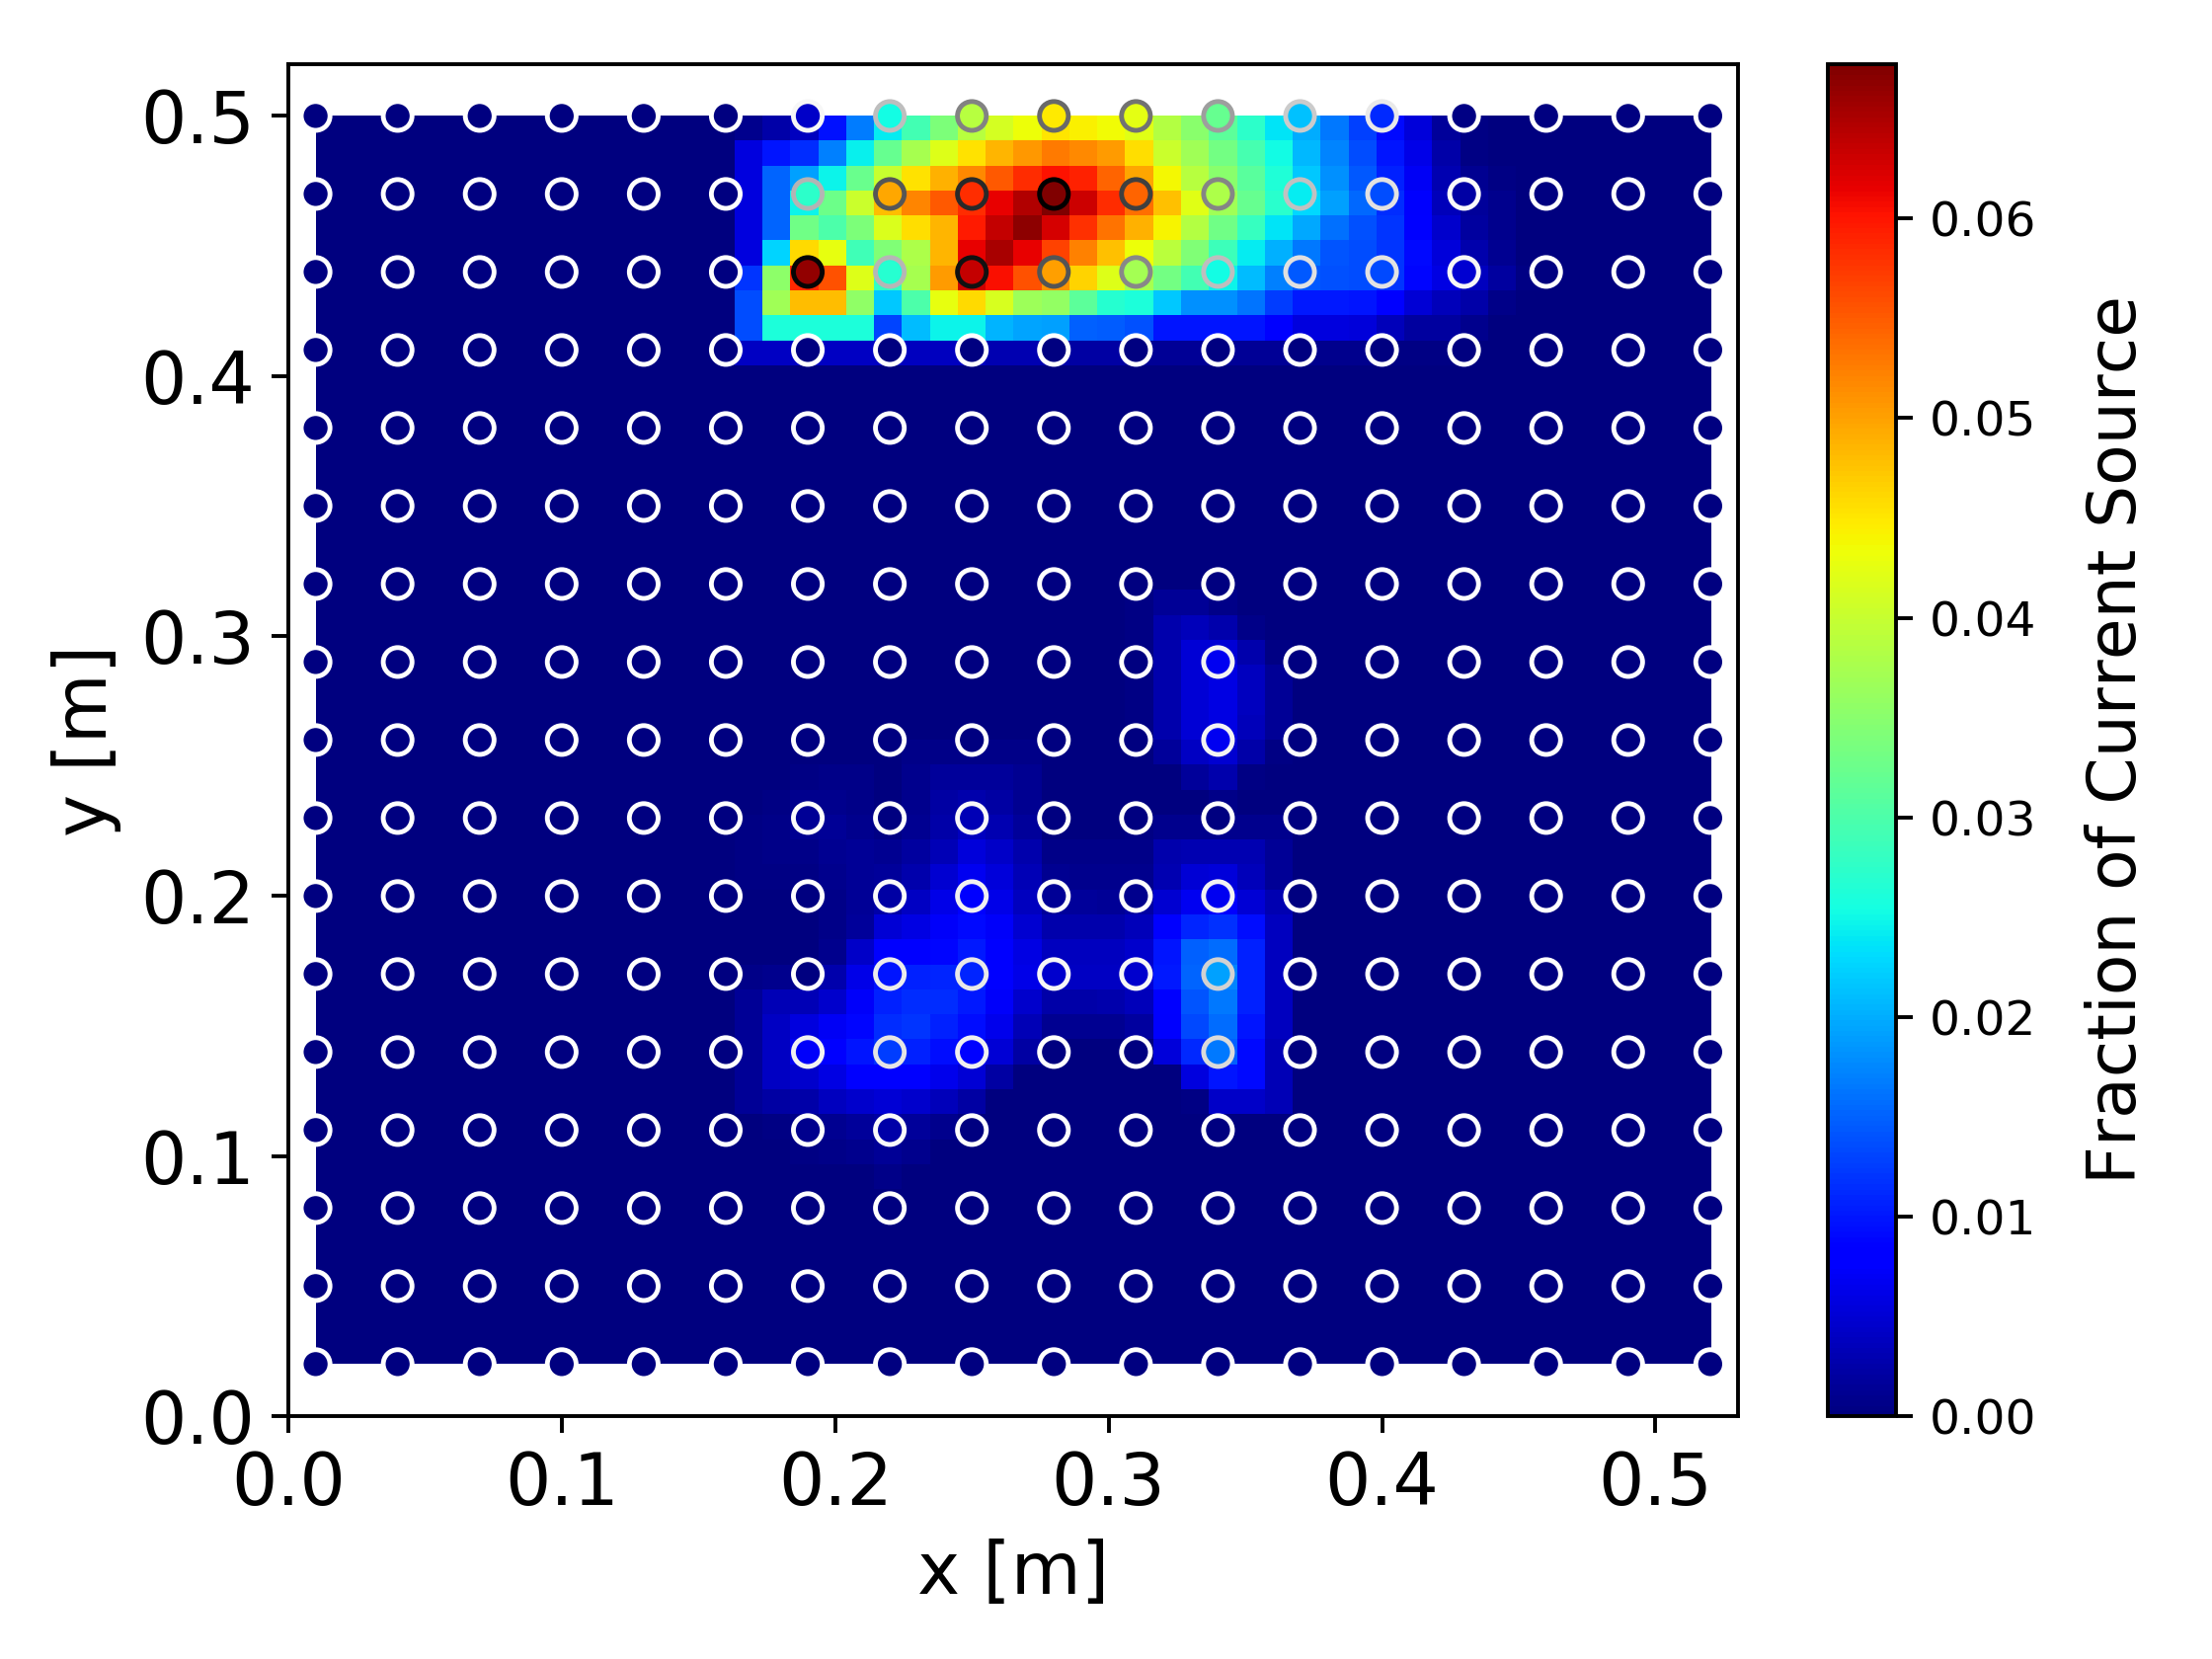
\includegraphics[width=8cm]{iCSDPlantSoil.png}}
\subcaptionbox{Comparison between laboratory and simulated MALM resistances. The simulation of the resistances bases on the inverted resistivity distribution (BERT) and estimated current source distribution.\label{PlantMalmCheck}}{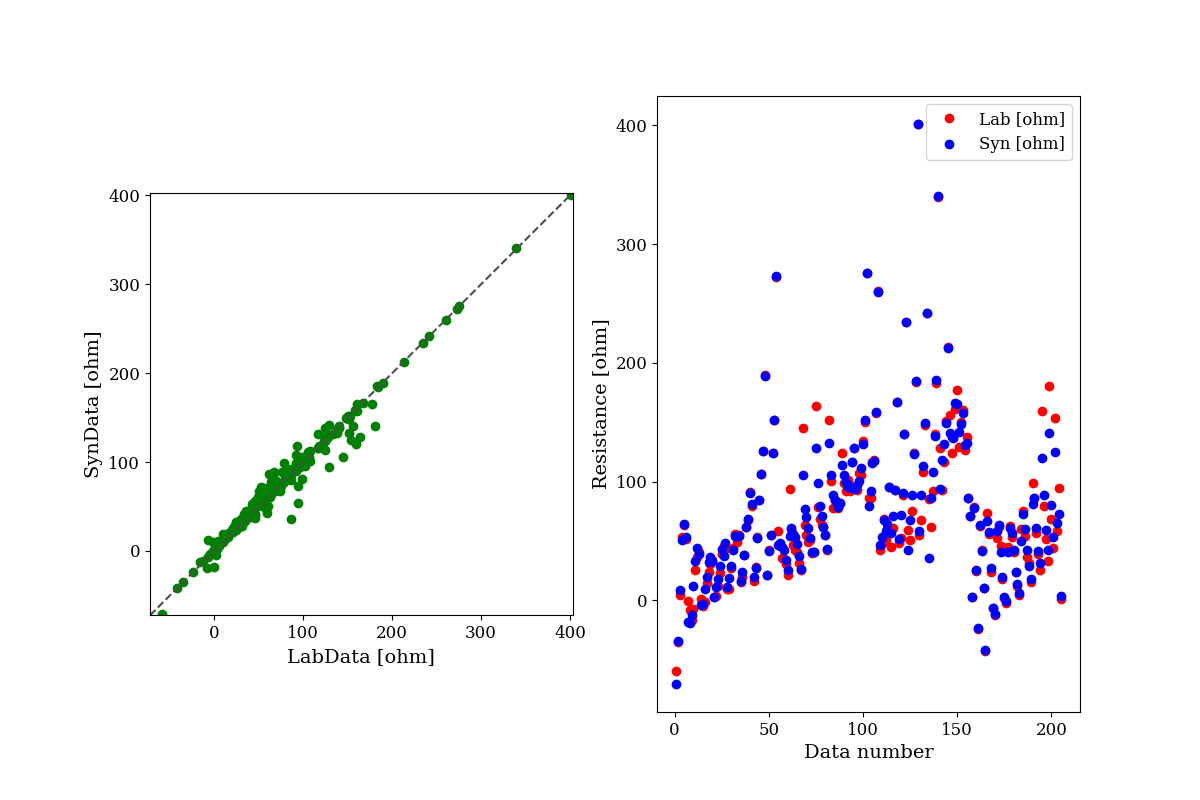
\includegraphics[width=8.5cm]{PlantMalmCheck.png}}
\caption{Experiment with maize plant in soil.\label{PlantMALM}}
\end{figure*}
\end{document}
